\documentclass[supercite]{Experimental_Report}

\title{~~~~~~计算机视觉实验二~~~~~~}
\author{崔昊阳}
\school{计算机科学与技术学院}
\classnum{CS2104}
\stunum{U202115415}
\instructor{刘康}
\date{2023年12月7日}

\usepackage{algorithm, multirow}
\usepackage{algpseudocode}
\usepackage{amsmath}
\usepackage{amsthm}
\usepackage{framed}
\usepackage{mathtools}
\usepackage{subcaption}
\usepackage{xltxtra}
\usepackage{bm}
\usepackage{tikz}
\usepackage{tikzscale}
\usepackage{pgfplots}
\usepackage{listings}
\lstset{
    backgroundcolor = \color{white},    % 背景色
    basicstyle = \small\ttfamily,           % 基本样式 + 小号字体
    rulesepcolor= \color{white},             % 代码块边框颜色
    breaklines = true,                  % 代码过长则换行
    numbers = left,                     % 行号在左侧显示
    numberstyle = \small,               % 行号字体
    keywordstyle = \color{blue}\bfseries,      % 关键字颜色
	identifierstyle=\color{purple}, 		% 标识符颜色
    commentstyle =\color{green},        % 注释颜色
    stringstyle = \color{green},          % 字符串颜色
    frame = None,                  % 用(带影子效果)方框框住代码块
    showspaces = false,                 % 不显示空格
    columns = flexible,                    % 字间距固定
}

\pgfplotsset{compat=1.16}

\newcommand{\cfig}[3]{
  \begin{figure}[H]
    \centering
    \includegraphics[width=#2\textwidth]{images/#1.tikz}
    \caption{#3}
    \label{fig:#1}
  \end{figure}
}

\newcommand{\sfig}[3]{
  \begin{subfigure}[b]{#2\textwidth}
    \includegraphics[width=\textwidth]{images/#1.tikz}
    \caption{#3}
    \label{fig:#1}
  \end{subfigure}
}

\newcommand{\xfig}[3]{
  \begin{figure}[H]
    \centering
    #3
    \caption{#2}
    \label{fig:#1}
  \end{figure}
}

\newcommand{\rfig}[1]{\autoref{fig:#1}}
\newcommand{\ralg}[1]{\autoref{alg:#1}}
\newcommand{\rthm}[1]{\autoref{thm:#1}}
\newcommand{\rlem}[1]{\autoref{lem:#1}}
\newcommand{\reqn}[1]{\autoref{eqn:#1}}
\newcommand{\rtbl}[1]{\autoref{tbl:#1}}

\algnewcommand\Null{\textsc{null }}
\algnewcommand\algorithmicinput{\textbf{Input:}}
\algnewcommand\Input{\item[\algorithmicinput]}
\algnewcommand\algorithmicoutput{\textbf{Output:}}
\algnewcommand\Output{\item[\algorithmicoutput]}
\algnewcommand\algorithmicbreak{\textbf{break}}
\algnewcommand\Break{\algorithmicbreak}
\algnewcommand\algorithmiccontinue{\textbf{continue}}
\algnewcommand\Continue{\algorithmiccontinue}
\algnewcommand{\LeftCom}[1]{\State $\triangleright$ #1}

\newtheorem{thm}{定理}[section]
\newtheorem{lem}{引理}[section]

\colorlet{shadecolor}{black!15}

\theoremstyle{definition}
\newtheorem{alg}{算法}[section]

\def\thmautorefname~#1\null{定理~#1~\null}
\def\lemautorefname~#1\null{引理~#1~\null}
\def\algautorefname~#1\null{算法~#1~\null}

\begin{document}

\maketitle

\clearpage

\pagenumbering{Roman}

\tableofcontents[level=2]

\clearpage

\pagenumbering{arabic}

\section{实验要求}
任务要求:设计一个卷积神经网络,并在其中使用 ResNet 模块,在 MNIST 数据集上实现 10 分类手写体数字识别。
注意事项:
\begin{enumerate}
	\item 深度学习框架任选。
	\item 不能直接导入现有的 ResNet 网络。
	\item 可以尝试不同的网络架构、激活函数、训练超参数等,至少尝试两种,观察并比较网络性能。
	\item 实验报告需包含神经网络架构、每一轮 mini-batch 训练后的模型在训练集和测试集上的损失、最终的训练集和测试集准确率,测试集十分类中每一类的准确率,不同设计变化导致的网络性能差异,以及对应的实验分析。
	\item 将代码和实验报告打包成 ZIP 压缩包,以“姓名-学号-实验报告\#”命名,比如“张三-2020XXX-实验报告一.zip”,提交到学习通。
	\item 截止时间为 12 月 27 号下午 2:00。
\end{enumerate}

\section{数据处理}
\subsection{数据集获取和数据探索}
本次实验的数据集是 MNIST 数据集。它由一个由 60000 张 $28\times 28\times 1$ 图像组成的训练集和由 10000 张 $28\times 28\times 1$ 图像组成的验证集构成。
每张图像都有且仅有一个手写的 0 到 9 之间的数字和一个图中数字的真实值标签。我们的任务是构建并训练模型,使其以尽可能高的准确率根据输入的图像预测其标签。

我们首先进行数据集的获取。我们通过互联网获取 MNIST 数据集。获取到的数据集由 4 个文件构成:\texttt{train-images.idx3-ubyte}, \texttt{train-labels.idx1-ubyte}, \texttt{t10k-images.idx3-ubyte} 和 \texttt{t10k-labels.idx1-ubyte}。
它们分别存储训练集的图片、训练集的标签、验证集的图片以及验证集的标签。由于数据集已经被划分成 60000 张图像的训练集和 10000 张图像的验证集,我们无需再进行数据集划分。
下面,我们将图像从文件中提取出来并和标签建立一一对应关系,以方便后续的数据探索和模型训练、测试。

我们编写了 \texttt{convert\_to\_img()} 函数来提取图像并建立图像和标签的一一对应关系。我们首先创建一个 \emph{MNIST} 目录用来存储这些图像和关系。
我们使用 \emph{MNIST/train} 和 \emph{MNIST/valid} 分别存放提取后的训练集图像和验证集图像。同时,我们还分别创建了 \emph{train.txt} 和 \emph{valid.txt} 文件
用于保存图像和标签的一一对应关系。这两个文件的每一行包括用空格分隔的两个字段,它们分别是图像的相对路径和图像的标签。这样,我们就可以通过读取这两个文件来依次找到
数据集的每个图像和它所对应的标签了。

接下来我们进行数据探索。经过观察,我们发现,所有的数据没有缺失或明显异常。所以我们无需进行数据清洗。
接下来,我们统计训练集和验证集中 10 类图像的个数,如图\ref{训练集数据个数分布图}和图\ref{验证集数据个数分布图}所示。
从图中我们可以看出,训练集每类图像的个数在 6000 张左右,验证集每类图像的个数在 1000 张左右。
10 类图像的个数差异较小,没有明显的类别不平衡现象。
\begin{figure}[H]
	\begin{center}
		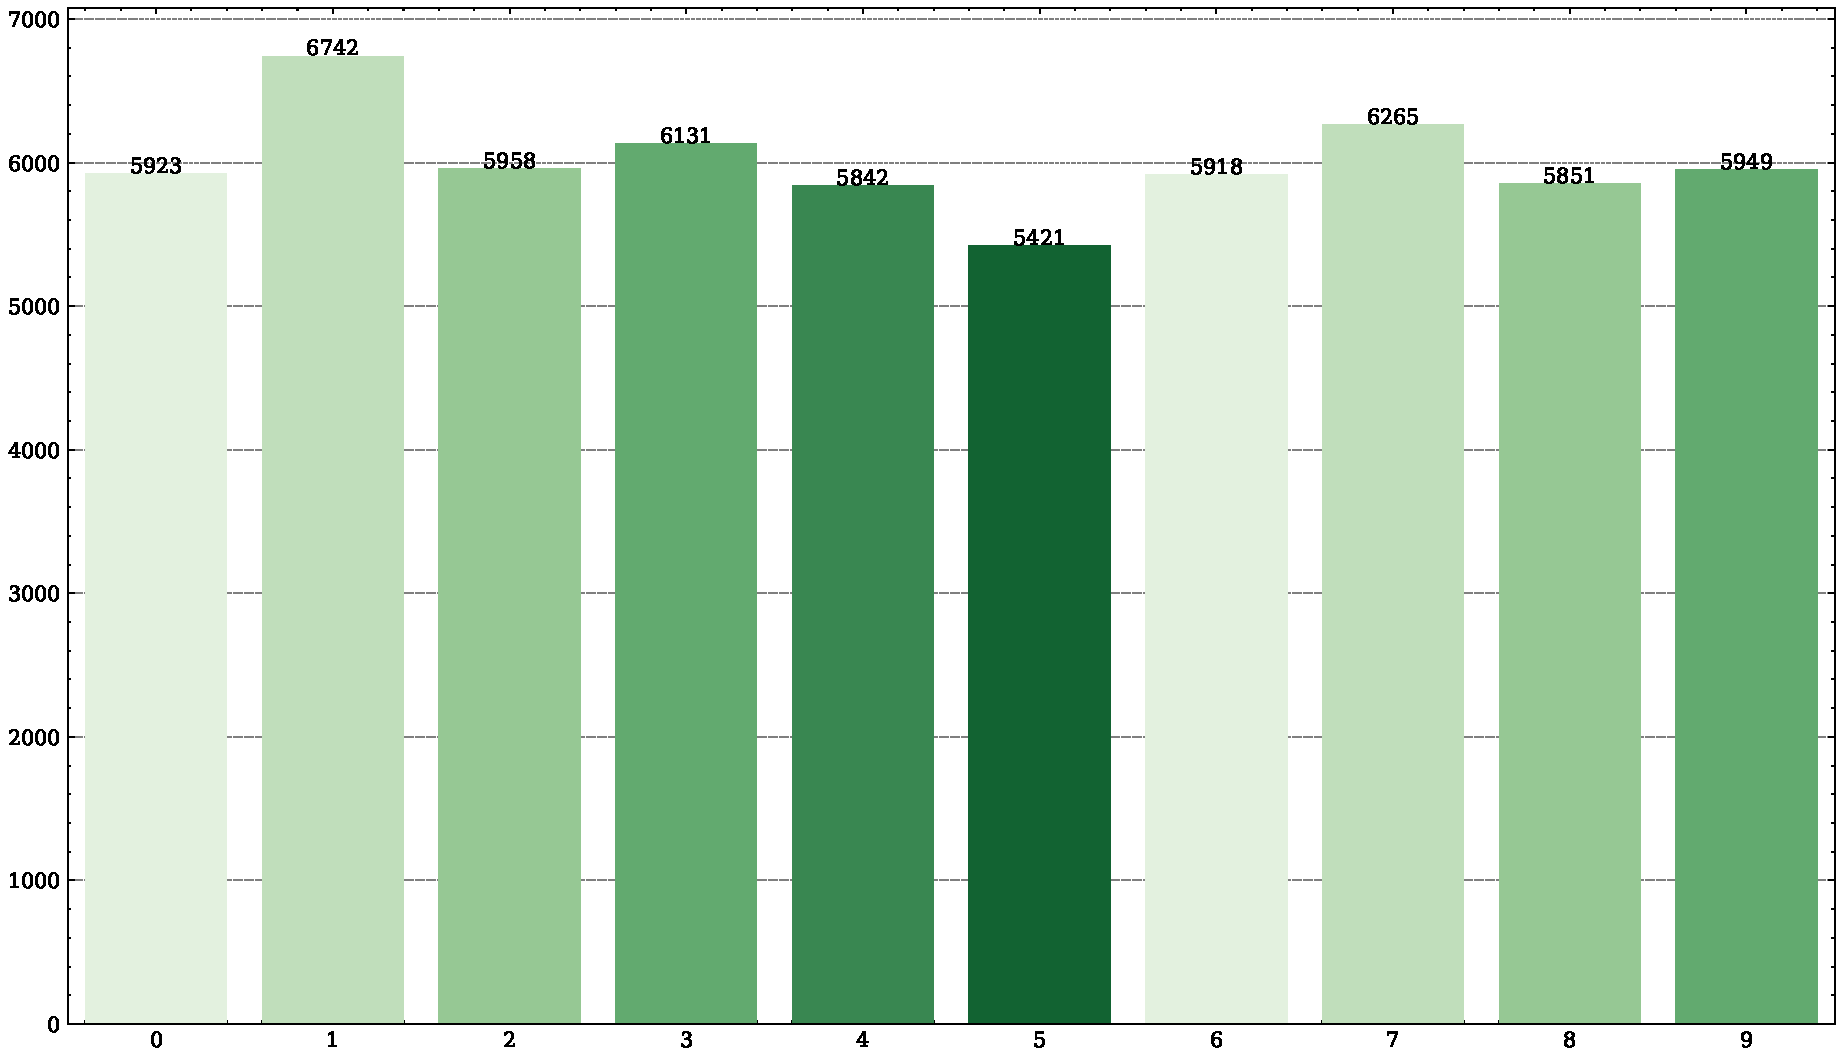
\includegraphics[scale=0.4]{../images/训练集数据个数分布图.pdf}
		\caption{训练集数据个数分布图}
		\label{训练集数据个数分布图}
	\end{center}
\end{figure}
\begin{figure}[H]
	\begin{center}
		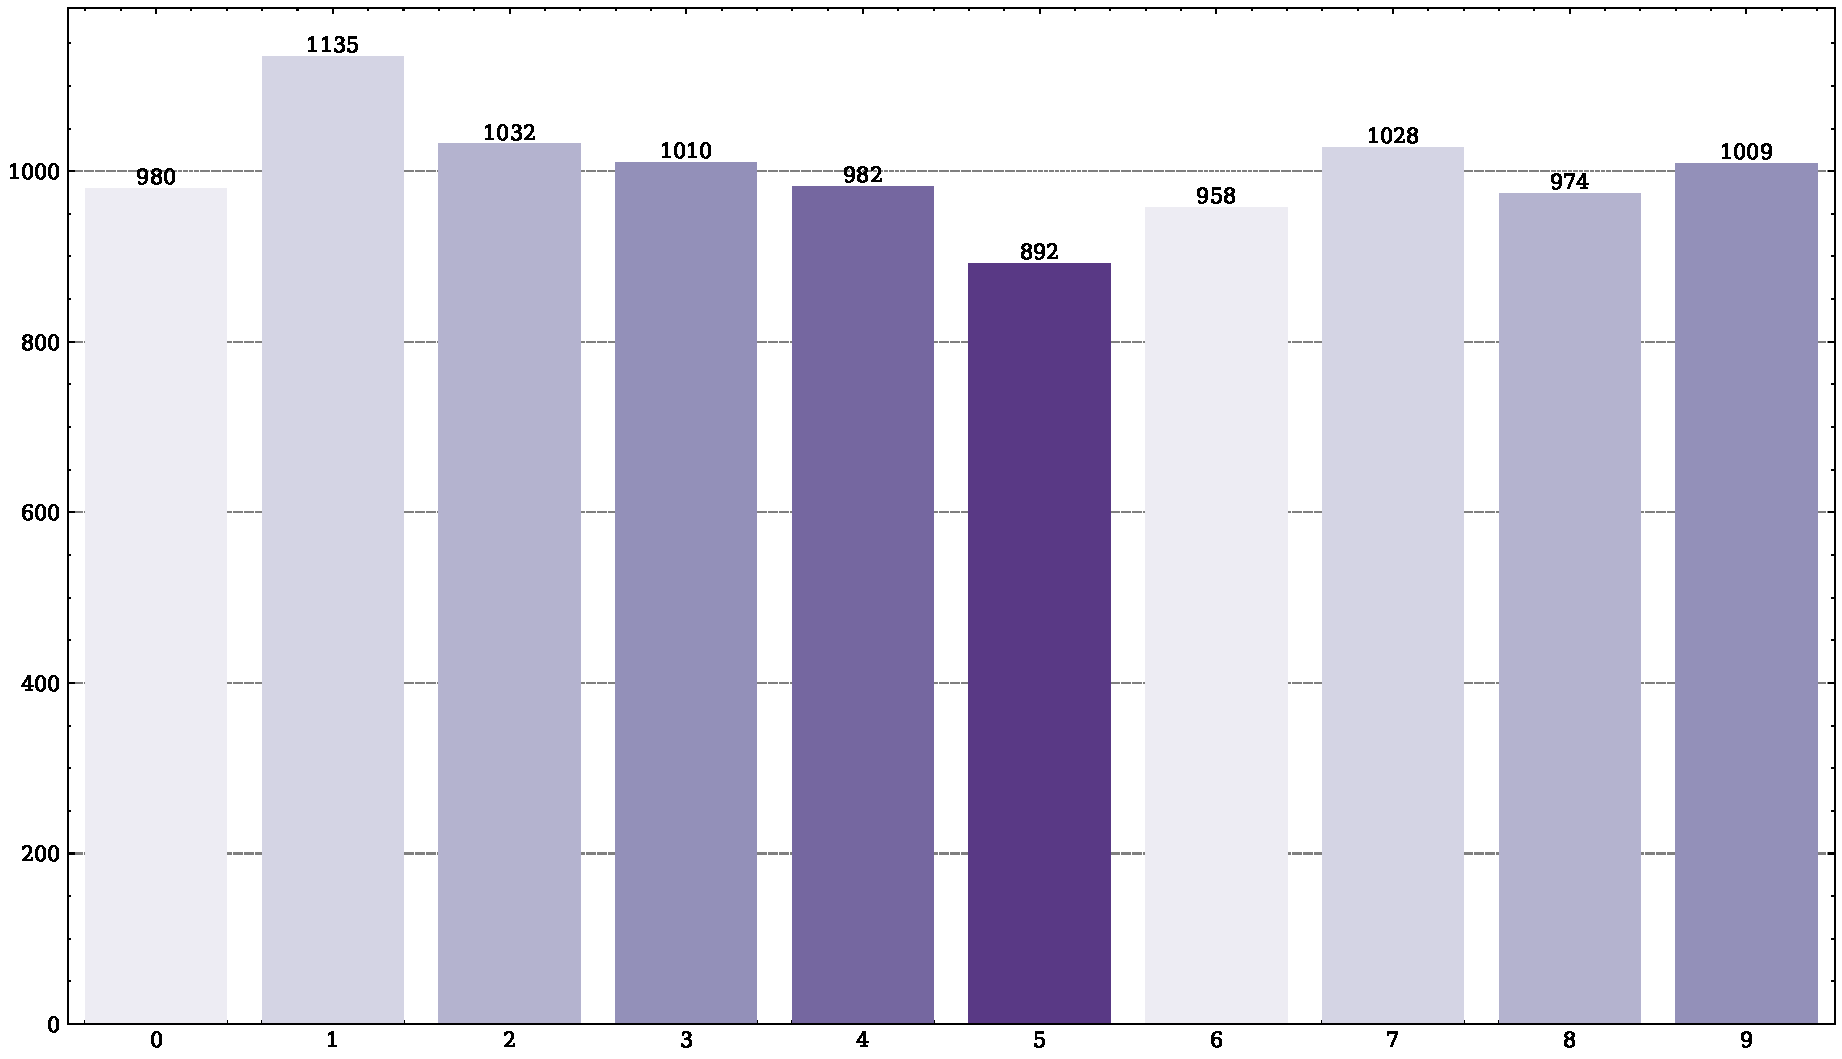
\includegraphics[scale=0.4]{../images/验证集数据个数分布图.pdf}
		\caption{验证集数据个数分布图}
		\label{验证集数据个数分布图}
	\end{center}
\end{figure}

\subsection{数据增强和 Dataset 的构建}

完成数据集的获取和数据探索后,我们进行数据增强和 Dataset 的构建。

数据增强是一种在深度学习中常用的技术,它通过对原始数据进行一系列随机变换和扩充,
生成新的训练样本,以增加训练数据的多样性和数量。数据增强可以提高模型的泛化能力、减轻过拟合,并改善模型在现实世界中的鲁棒性。
在本次实验中,由于数字在图像中的位置和其标签无关,我们采用随机裁剪的方式进行数据增强。为了使模型易于训练,我们还对输入的图像进行了标准化。
我们计算了 ImageNet 数据集中所有的图像所有通道的均值和标准差,并将其作为数据标准化和的均值和标准差。训练集和验证集上的数据增强方法如下。
\begin{lstlisting}[language=python]
norm_mean = [0.449]  # ImageNet 中所有图像的平均值
norm_std = [0.226]  # ImageNet 中所有图像的标准差
# 训练集数据增强
train_transform = transforms.Compose([
    transforms.RandomCrop(28, padding=4),
    transforms.ToTensor(),
    transforms.Normalize(norm_mean, norm_std),
])
# 验证集数据增强
valid_transform = transforms.Compose([
    transforms.ToTensor(),
    transforms.Normalize(norm_mean, norm_std),
])
\end{lstlisting}

最后,我们编写了一个支持迭代的数据集类,用于将上述数据集转换成可输入模型的形式。这个类的实例在每次迭代过程中,会读取 txt 文件中的一行。
提取这一行中图片的地址和标签并找到图像,对图像进行数据增强后转为 tensor,最终返回包含增强后的图像和标签的二元组。

至此,数据处理完成。

\section{模型架构}
接下来,我们进行模型架构的设计。在本实验中,我们一共设计了两个模型架构,并均进行了测试。
\subsection{网络结构}
根据实验要求,网络应为一个包含残差块的卷积神经网络。我们设计了两种带有残差块的网络架构。它们分别是 LeNet\_RB 和 ResNet18。
下面,我们首先介绍残差块的结构,再分别介绍两种网络的结构。

残差块包括两个分支:left 和 shortcut。其中,left 分支由两个卷积层、两个批归一化层和一个 ReLU 激活函数层组成。
shortcut 分支由一个卷积层和一个批归一化层。层的输出是输入经两个分支映射后的结果之和。残差块的结构如图\ref{残差块网络结构图}
所示。
\begin{figure}[H]
	\begin{center}
		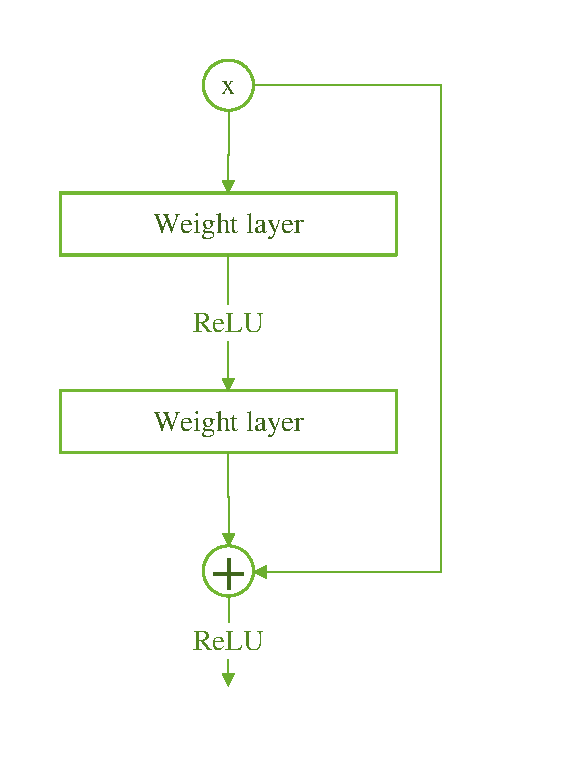
\includegraphics[scale=0.7]{../images/残差块网络结构图.pdf}
		\caption{残差块网络结构图}
		\label{残差块网络结构图}
	\end{center}
\end{figure}

LeNet\_RB 是 LeNet5 网络和一个残差块组成的。我们将一个残差块放到 LeNet5 的卷积层和全连接层之间,即可得到 LeNet\_RB。
LeNet\_RB 的网络结构图如图\ref{LeNetRB网络结构图}所示。该网络的参数较少,所以训练时间和推理时间较短,适合于简单的图像分类任务。
\begin{figure}[H]
	\begin{center}
		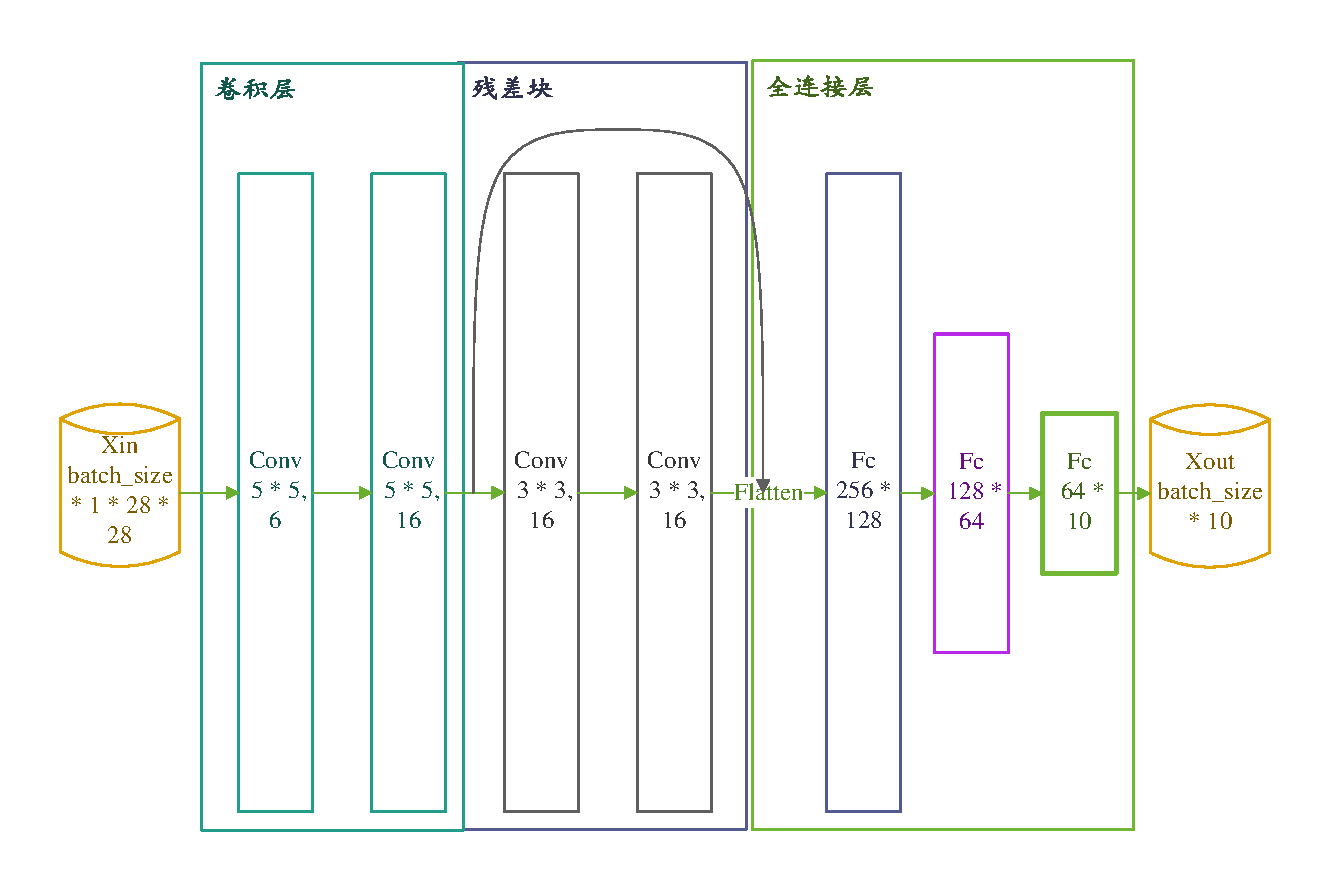
\includegraphics[scale=0.45]{../images/LeNetRB网络结构图.pdf}
		\caption{LeNet\_RB 网络结构图}
		\label{LeNetRB网络结构图}
	\end{center}
\end{figure}

ResNet18 是 ResNet 的最小版本,它由 18 个层组成。ResNet18 包含 1 个卷积层、4 个残差连接层、1个池化层和 1 个全连接层。其中, 1 个残差连接层由 2 个残差块连接而成。
ResNet18 的网络结构图如图\ref{ResNet18网络结构图}所示。该网络的参数较多,可以本实验中达到更高的准确率,但是训练和推理时间较长。
\begin{figure}[H]
	\begin{center}
		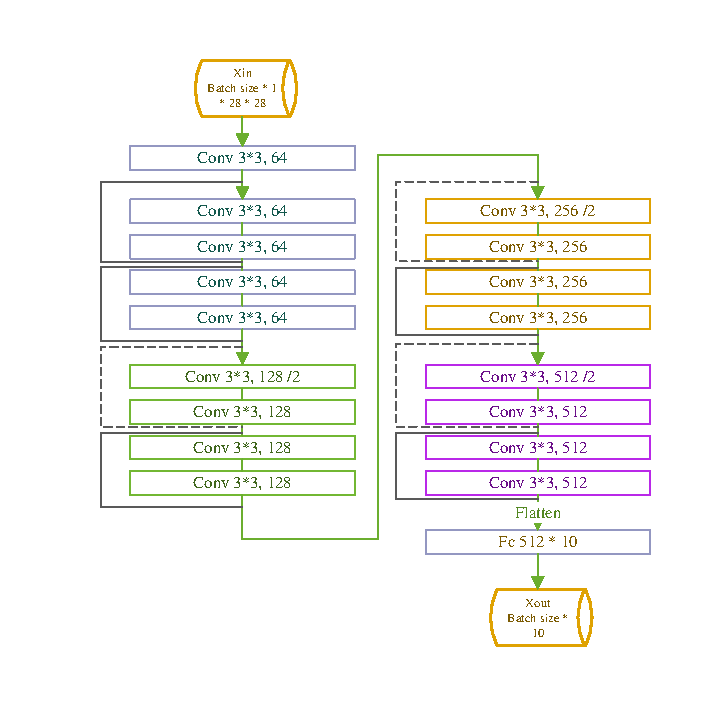
\includegraphics[scale=0.9]{../images/ResNet18网络结构图.pdf}
		\caption{ResNet18 网络结构图}
		\label{ResNet18网络结构图}
	\end{center}
\end{figure}

\subsection{损失函数}
损失函数是度量当前分类器的输出和真实值的差异的函数。
本实验要求完成一个 10 分类任务。所以,我们使用交叉熵损失来作为我们的损失函数。
交叉熵是一种多分类任务中常用的损失函数。假设分类器的输出向量 $p\in R^c$,
真实值的独热向量为 $q\in R^c$。那么交叉熵 $H(p, q)$ 的计算公式如下。
$$
H(p, q)=-\sum_{i=1}^{c}p_i log(q_i)
$$

% 除此之外,我们还在损失函数中加入了正则化项。在实验中,我们尝试了 L1 正则化和 L2 正则化两种方法,最终选择了 L1 正则化方法。
% 下面我们将介绍这两种正则化方法。

% L1 正则化通过在损失函数中添加参数的 1-范数来对参数进行约束。
% 通过 L1 正则化,我们可以得到稀疏的模型参数矩阵,从而实现模型简化和特征选择。L1 正则化 $L1$ 的计算公式如下。
% $$
% L1=\lambda \sum_{i=1}^n |w_i|
% $$
% 其中,$\lambda$ 是用来调节正则化强度的系数,$w$ 是模型参数矩阵。

% L2 正则化通过在损失函数中添加参数的 2-范数来对参数进行约束。
% 通过 L2 正则化,我们使参数的绝对值减小,从而缓解过拟合现象。L2 正则化 $L2$ 的计算公式如下。
% $$
% L2=\lambda \sum_{i=1}^n w_i^2
% $$
% 其中,$\lambda$ 是用来调节正则化强度的系数,$w$ 是模型参数矩阵。

% 综上所述,我们的损失函数计算公式如下:
% $$
% Loss(p, q) = -\sum_{i=1}^{c}p_i log(q_i)+\lambda \sum_{i=1}^n |w_i|
% $$

\subsection{优化器}
优化器用来决定下一步模型的参数如何变化。在本实验中,我们选用 AdamW 优化器。
AdamW 优化器是 Adam 优化器的改进版本。它在 Adam 优化器的基础上增加了权值衰减功能。
Adam 优化器同时考虑指数移动平均的一阶动量和二阶动量以指导参数更新。其计算公式如下。
$$
\begin{aligned}
	m_t&=\beta_1m_{t-1}+(1-\beta_1)g_t\\
	v_t&=\beta_2v_{t-1}+(1-\beta_2)diag(g_t^2)\\
	w_{t+1}&=w_{t}-\alpha\frac{m_t}{\sqrt{v_t}+\epsilon}
\end{aligned}
$$

其中,$m_t, v_t$ 是动量相关参数,$\alpha$ 为学习率,$w_t$ 是参数矩阵,$g_t$ 是梯度。
而 Adamw 优化器在 Adam 优化器的基础上加入了权值衰减系数,$w$ 矩阵的更新公式变为。
$$
w_{t+1}=(1-\lambda \alpha)w_{t}-\alpha\frac{m_t}{\sqrt{v_t}+\epsilon}
$$

由于 AdamW 优化器已经进行了学习率自适应,在本次实验中我们向优化器中传入固定值的学习率,而不在设置
学习率更新策略,使其随训练轮数发生变化。

至此,网络架构设计完成。


\section{实验结果}
\subsection{实验环境}
本实验在一个运算服务器上进行,服务器的配置如表\ref{服务器配置}所示。
\begin{table}[H]
	\centering
	\caption{实验环境表}
	  \begin{tabular}{c|c|c}
		\toprule
	  \multirow{3}[0]{*}{硬件} & CPU   & AMD EPYC 7551P 32-Core Processor \\
			& 内存大小    & 440G \\
			& GPU   & NVIDIA GeForce RTX 3090 \\\hline
	  \multirow{3}[0]{*}{软件} & 操作系统  & Ubuntu 20.04.5 LTS \\
			& 深度学习框架 & PyTorch 1.13.1 \\
			& IDE   & Vscode \\\bottomrule
	  \end{tabular}
	\label{服务器配置}
\end{table}
\subsection{超参数设置}
在本次实验中,为了使结果可复现,我们将随机数种子固定为 1024。我们还使用了 GPU 加速训练。

在网络架构方面,我们训练了 LeNet\_RB, ResNet18 两种网络。网络的架构已在上文中介绍。两种网络的输入均为一批 $28\times 28\times 1$
的矩阵,输出为相同数量的预测标签。

在训练方面,我们训练了 100 个 epoch。batch size 设置为 600。学习率设置为 $10^{-4}$。

对于优化器,我们选择了 AdamW 优化器,$\beta_1$ 参数为 0.9,$\beta_2$ 参数为 0.999。

\subsection{结果}
首先,我们使用上述的超参数对模型进行了训练,在完成每一轮训练后我们将模型在验证集上进行验证。验证所使用的评价指标
包括准确率和 macro f1 分数。我们选择验证集上准确率最高的模型参数进行保存。

在训练过程中,对于 LeNet\_RB模型,每个 mini\_batch 上训练集损失函数值变化和评价指标变化
如图\ref{LeNetRB训练损失函数batch}和图\ref{LeNetRB训练评价指标batch}所示;
每个 epoch 结束后训练集和验证集上的损失函数如图\ref{LeNetRB训练验证损失函数}所示;
每个 epoch 结束后训练集和验证集上的评价指标(准确率和 macro f1 分数)如图\ref{LeNetRB训练验证acc}和图\ref{LeNetRB训练验证f1}所示。
\begin{figure}[H]
	\begin{center}
		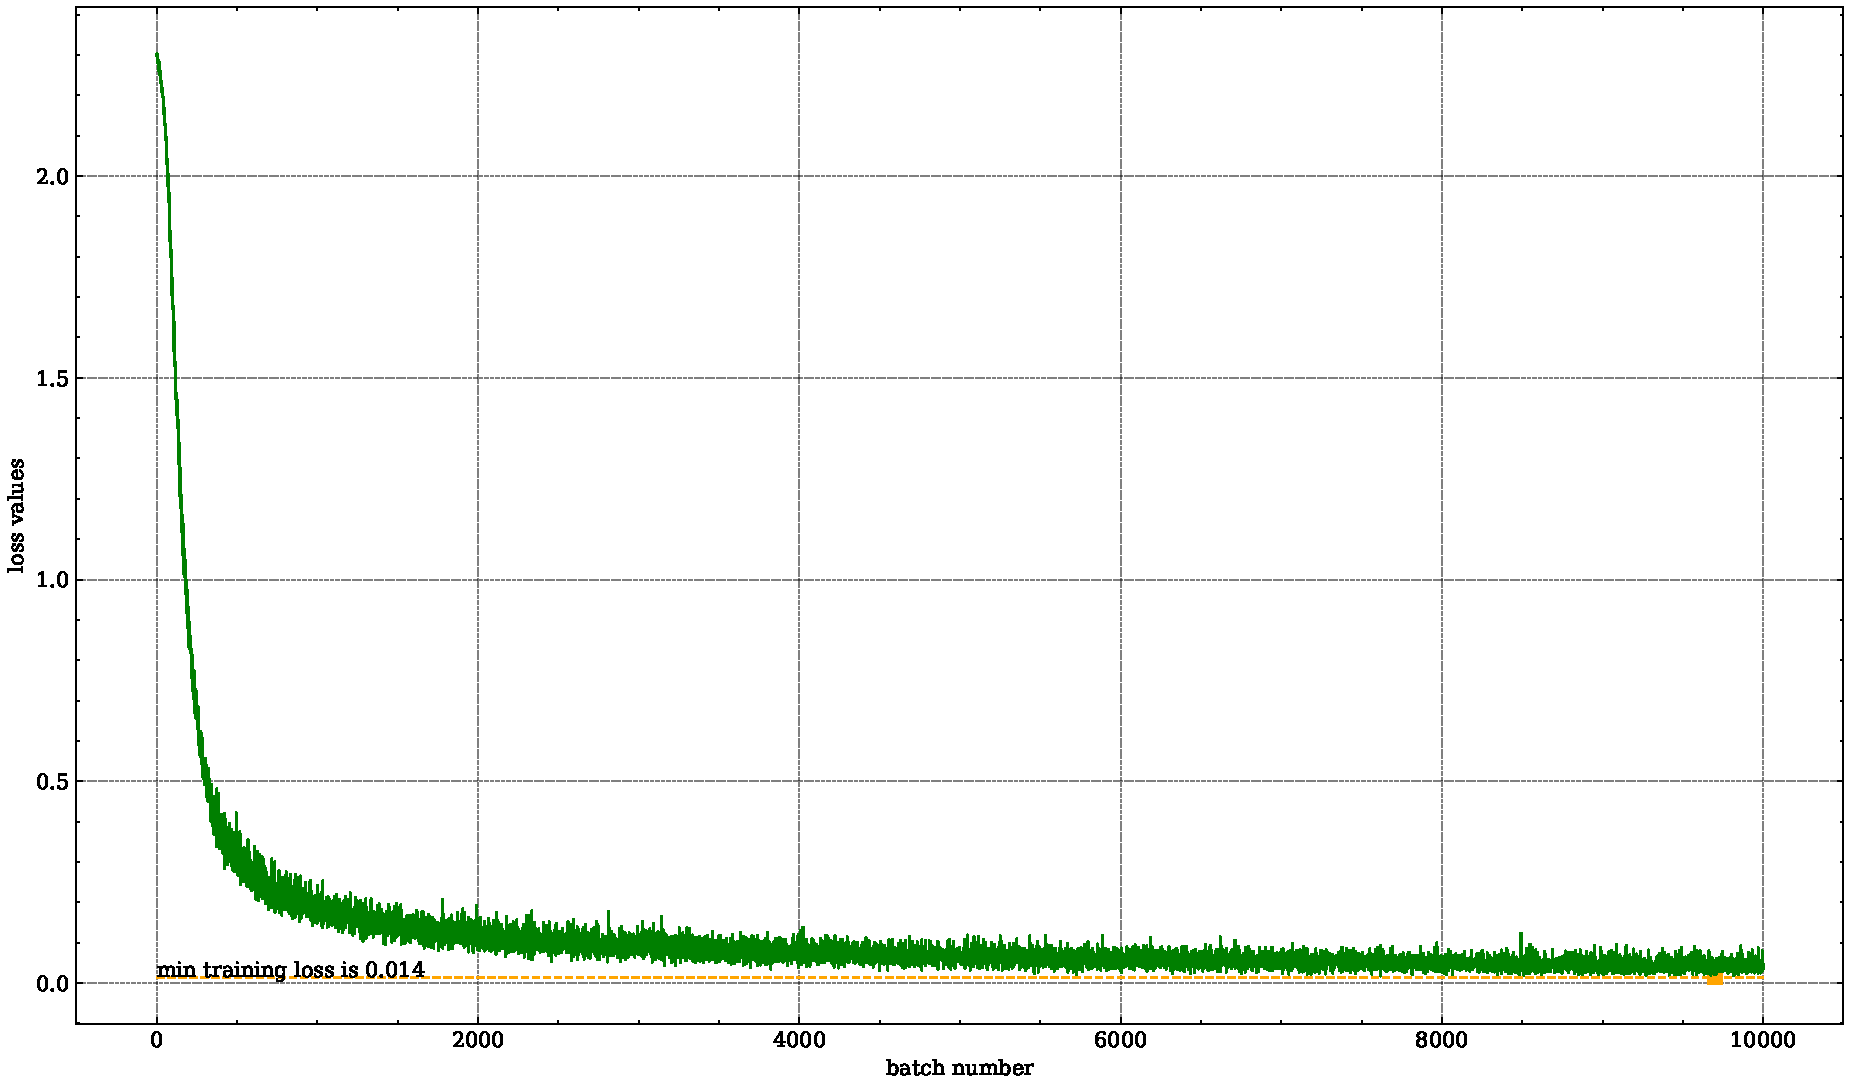
\includegraphics[scale=0.45]{../images/LeNetRB训练损失函数batch.pdf}
		\caption{LeNet\_RB训练损失函数变化图}
		\label{LeNetRB训练损失函数batch}
	\end{center}
\end{figure}
\begin{figure}[H]
	\begin{center}
		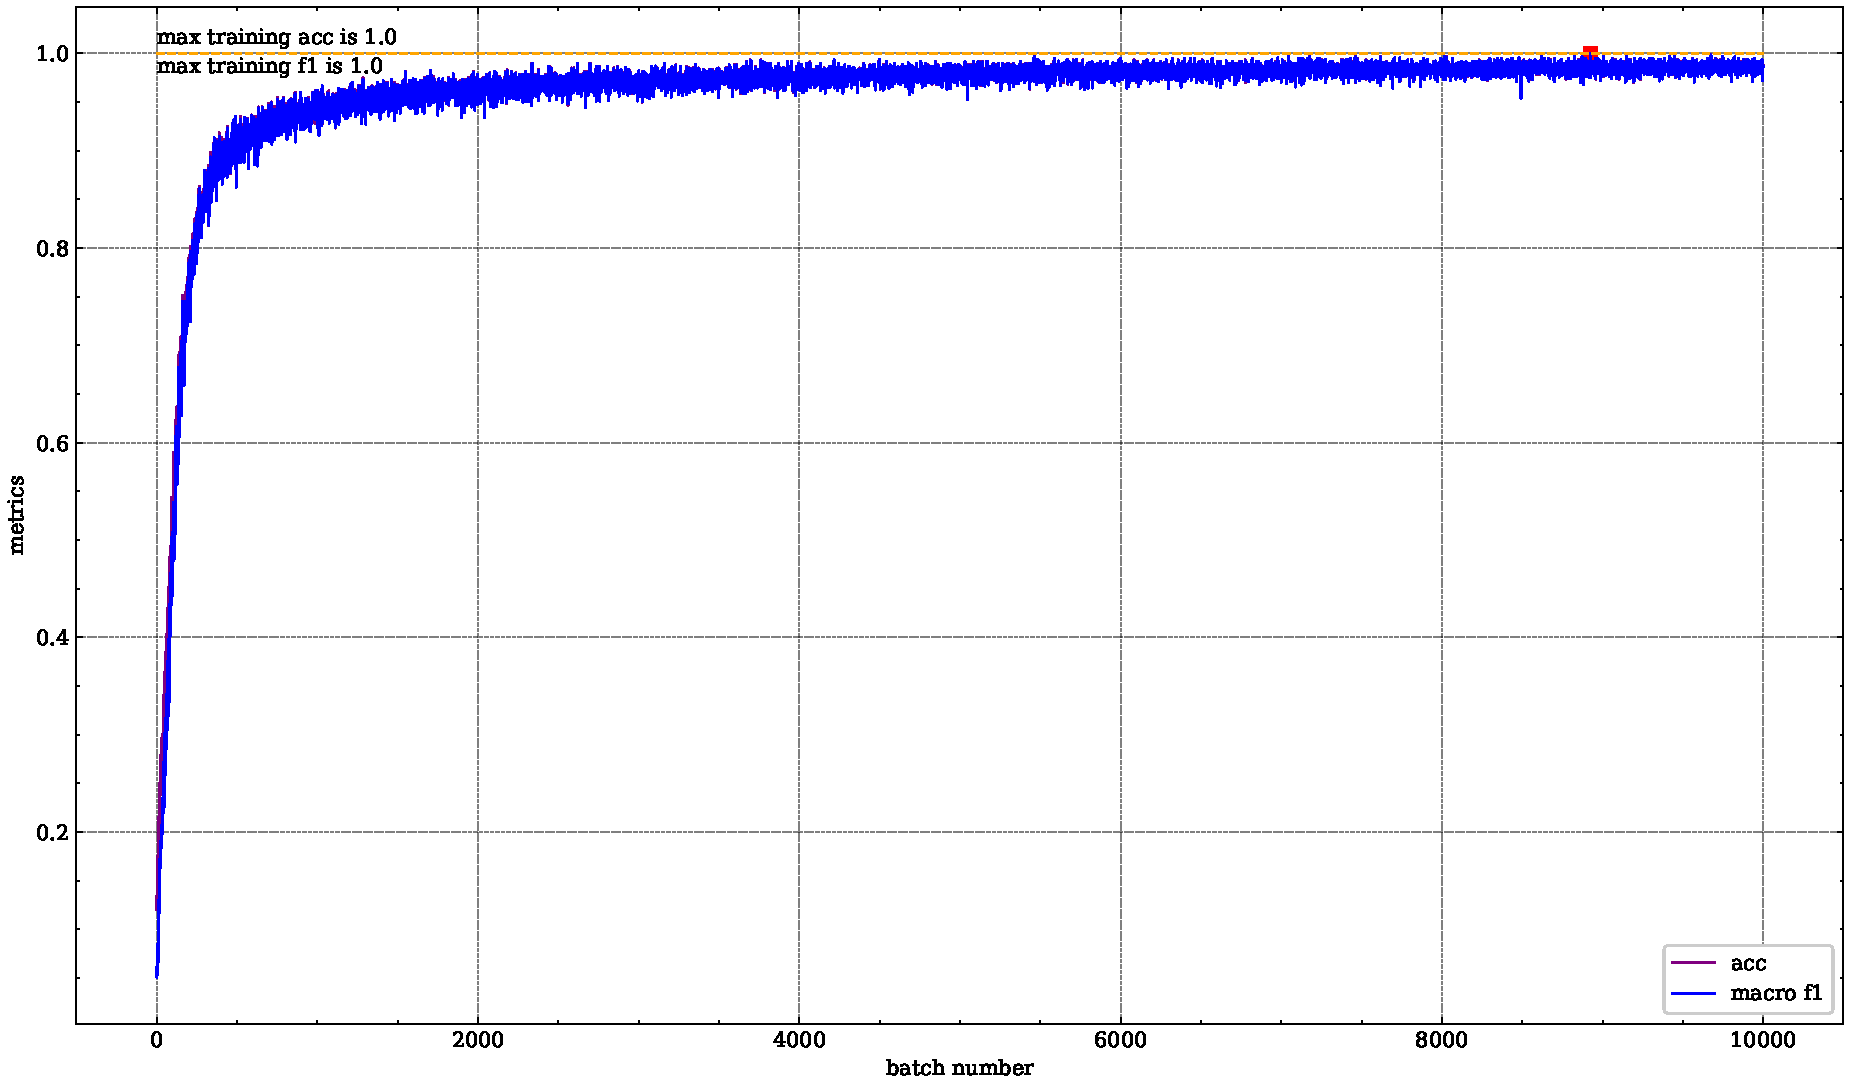
\includegraphics[scale=0.45]{../images/LeNetRB训练评价指标batch.pdf}
		\caption{LeNet\_RB训练评价指标变化图}
		\label{LeNetRB训练评价指标batch}
	\end{center}
\end{figure}
\begin{figure}[H]
	\begin{center}
		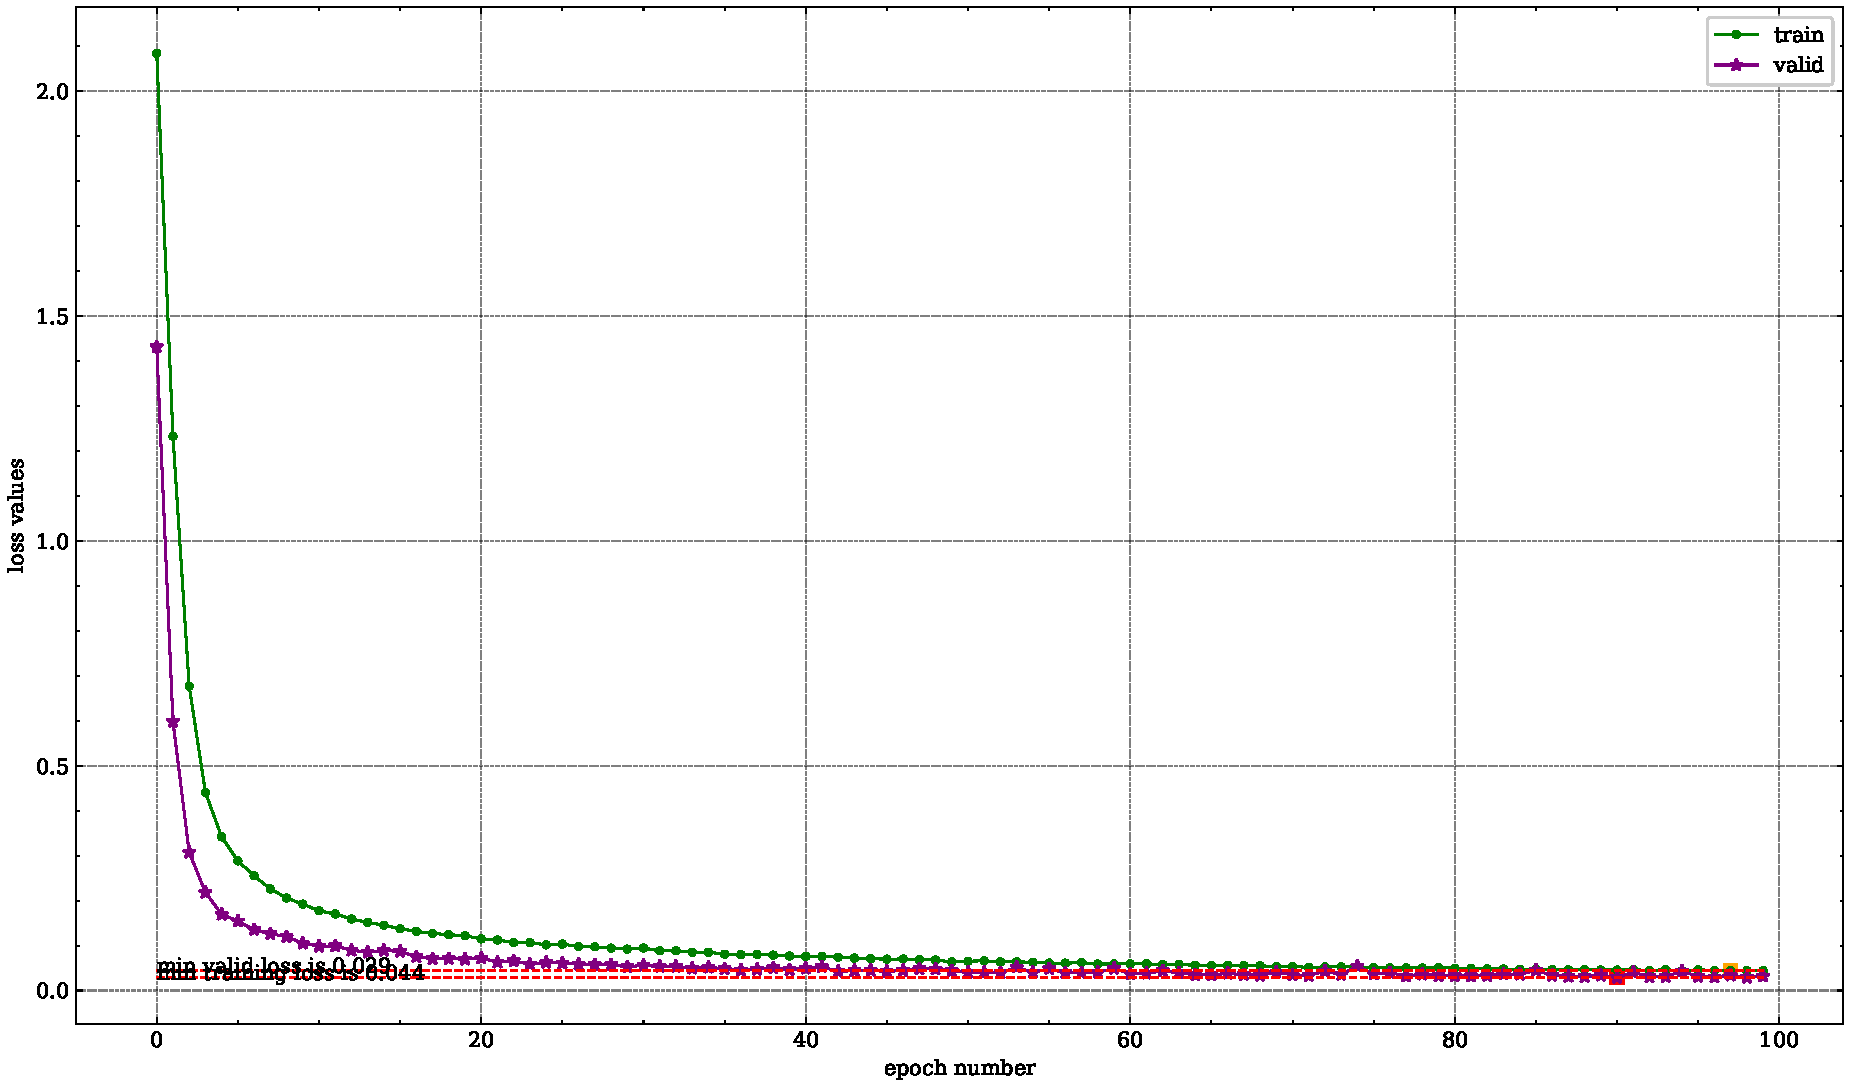
\includegraphics[scale=0.45]{../images/LeNetRB训练验证损失函数.pdf}
		\caption{LeNet\_RB 训练损失函数变化图}
		\label{LeNetRB训练验证损失函数}
	\end{center}
\end{figure}
\begin{figure}[H]
	\begin{center}
		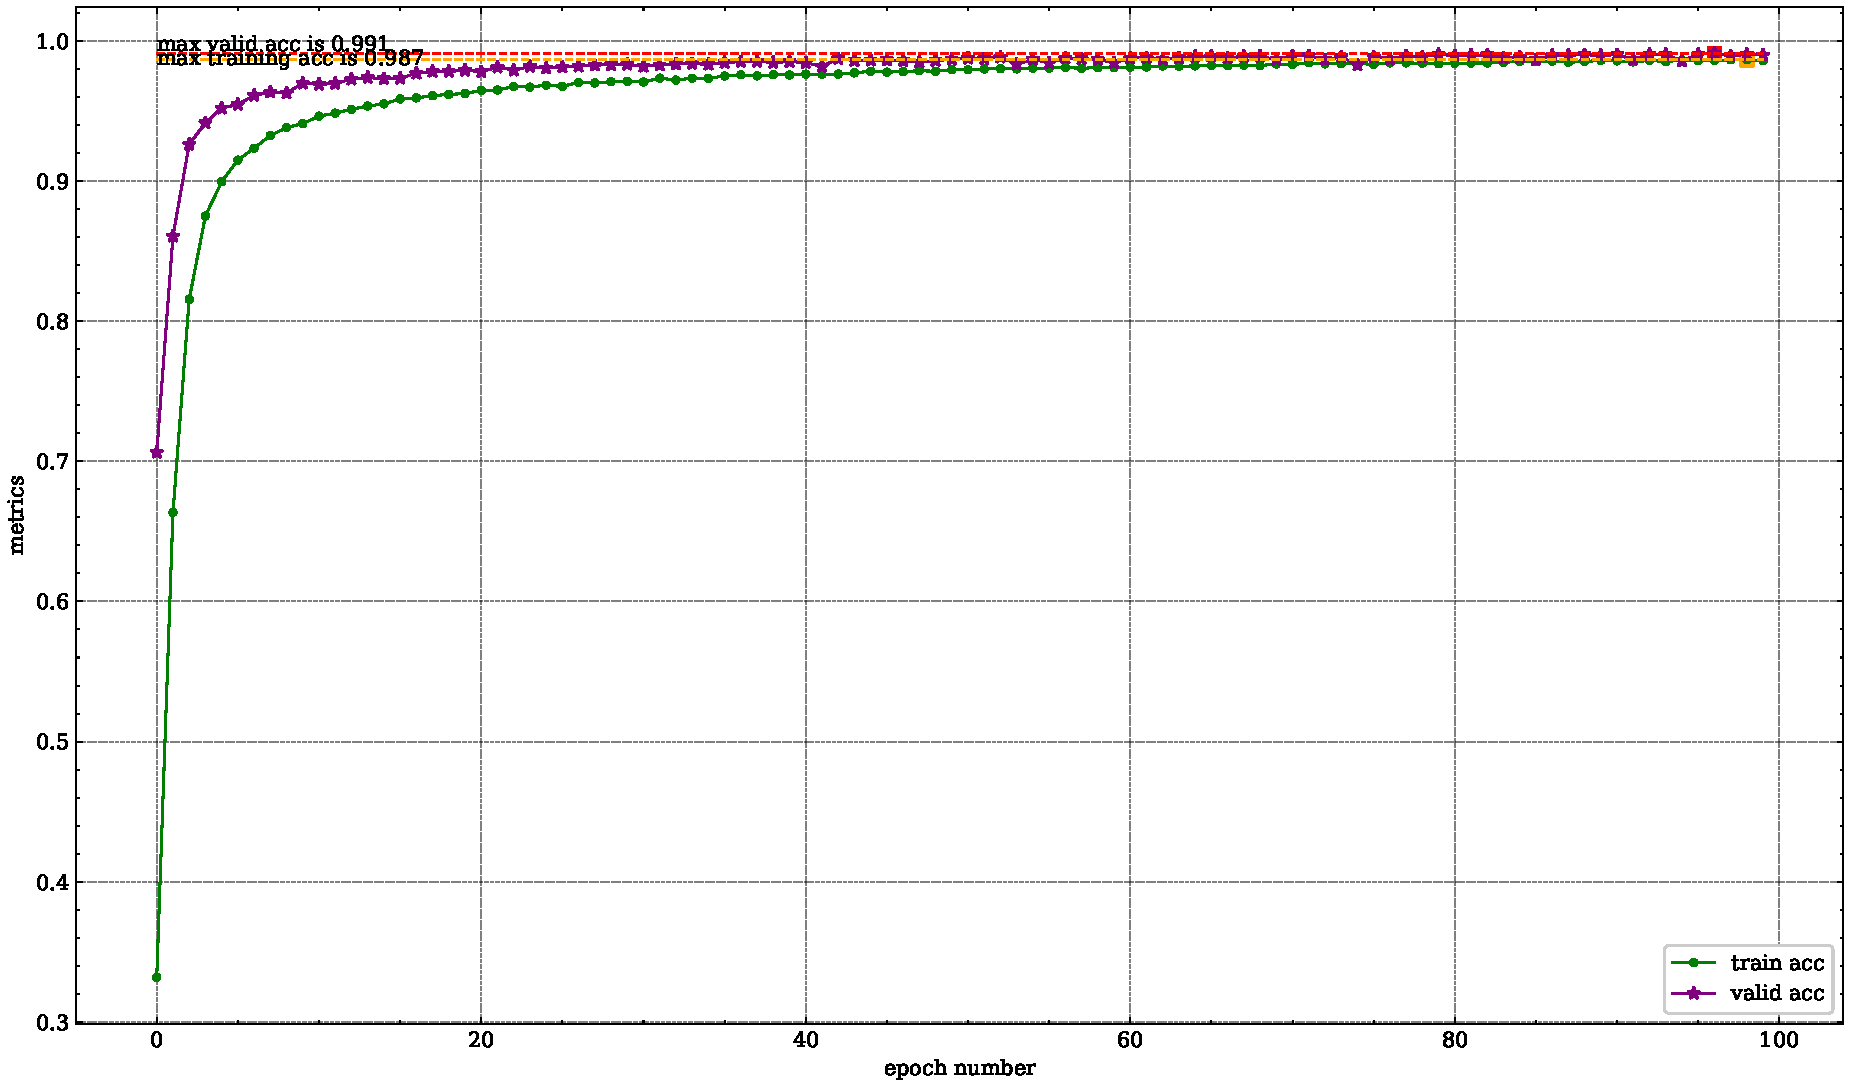
\includegraphics[scale=0.45]{../images/LeNetRB训练验证acc.pdf}
		\caption{LeNet\_RB 验证准确率变化图}
		\label{LeNetRB训练验证acc}
	\end{center}
\end{figure}
\begin{figure}[H]
	\begin{center}
		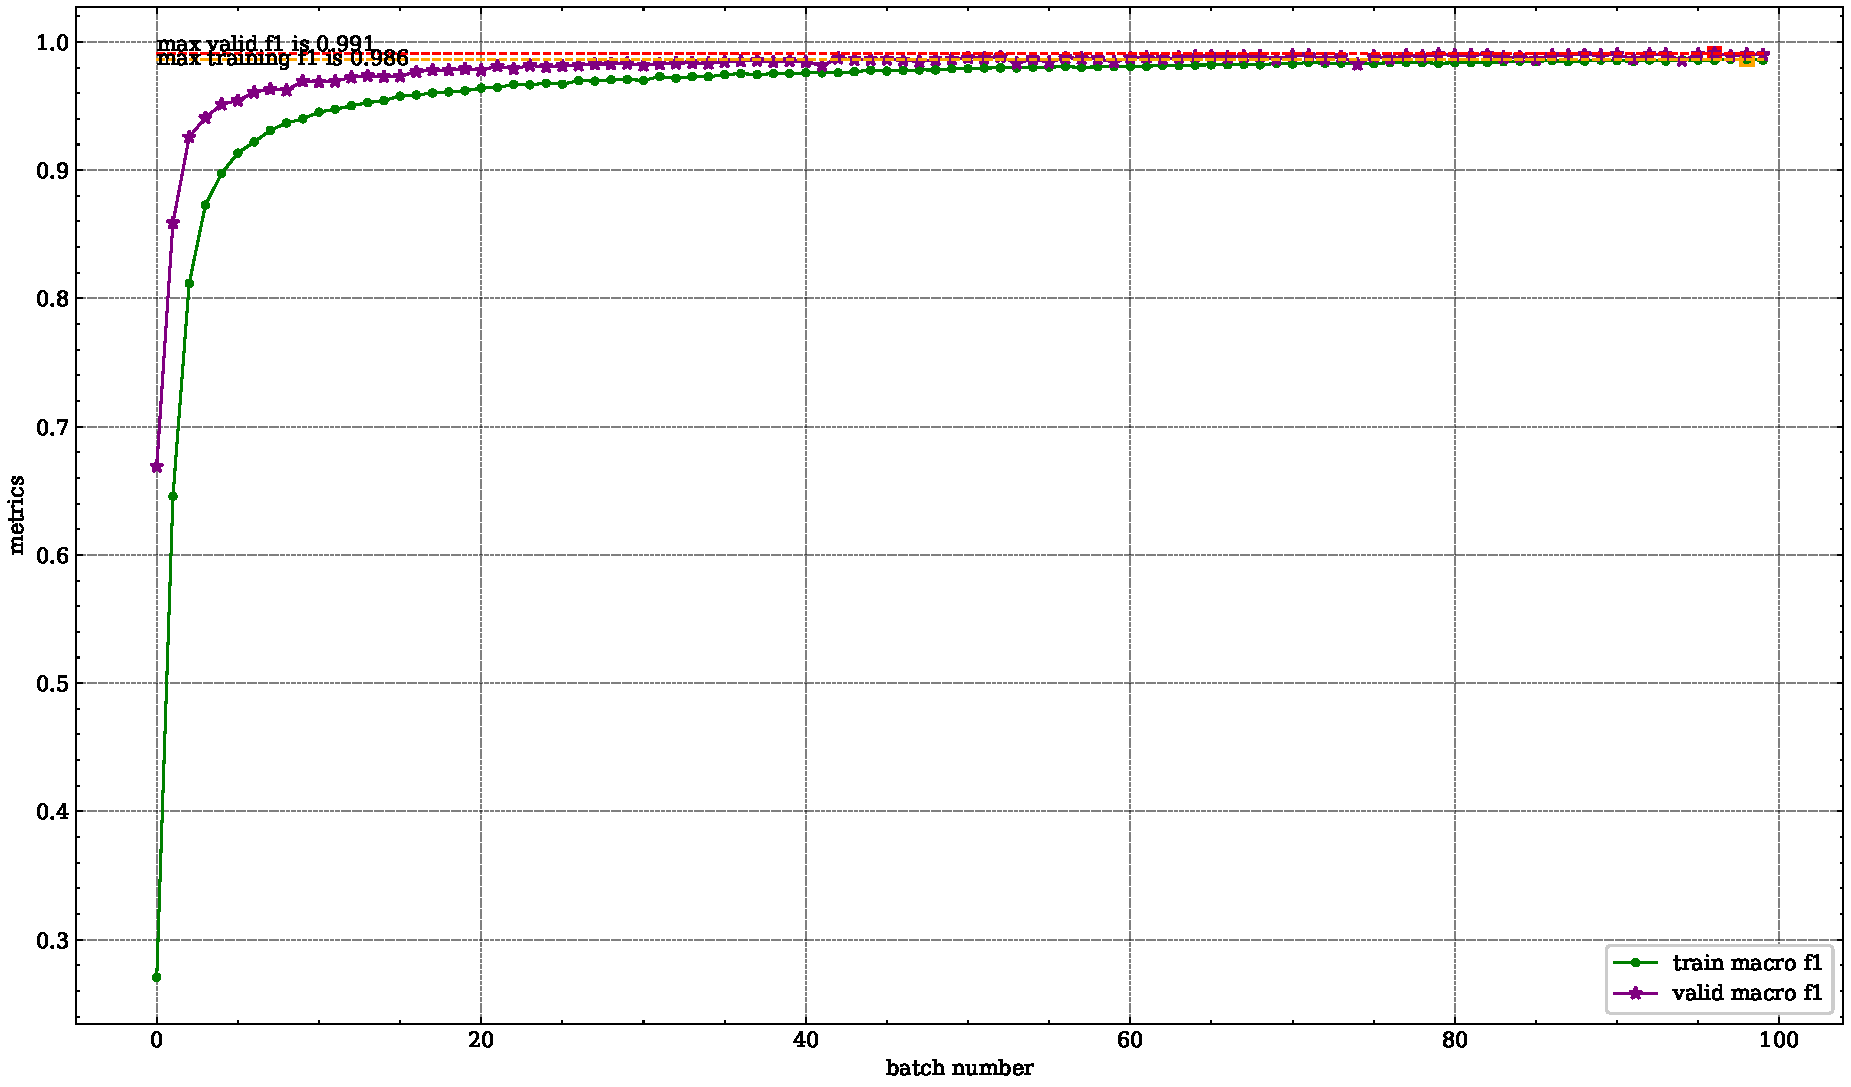
\includegraphics[scale=0.45]{../images/LeNetRB训练验证f1.pdf}
		\caption{LeNet\_RB 验证 macro f1 分数变化图}
		\label{LeNetRB训练验证f1}
	\end{center}
\end{figure}

对于 ResNet18 模型,每个 mini\_batch 上训练集损失函数值变化和评价指标变化
如图\ref{ResNet18训练损失函数batch}和图\ref{ResNet18训练评价指标batch}所示;
每个 epoch 结束后训练集和验证集上的损失函数如图\ref{ResNet18训练验证损失函数}所示;
每个 epoch 结束后训练集和验证集上的评价指标(准确率和 macro f1 分数)如图\ref{ResNet18训练验证acc}和图\ref{ResNet18训练验证f1}所示。
\begin{figure}[H]
	\begin{center}
		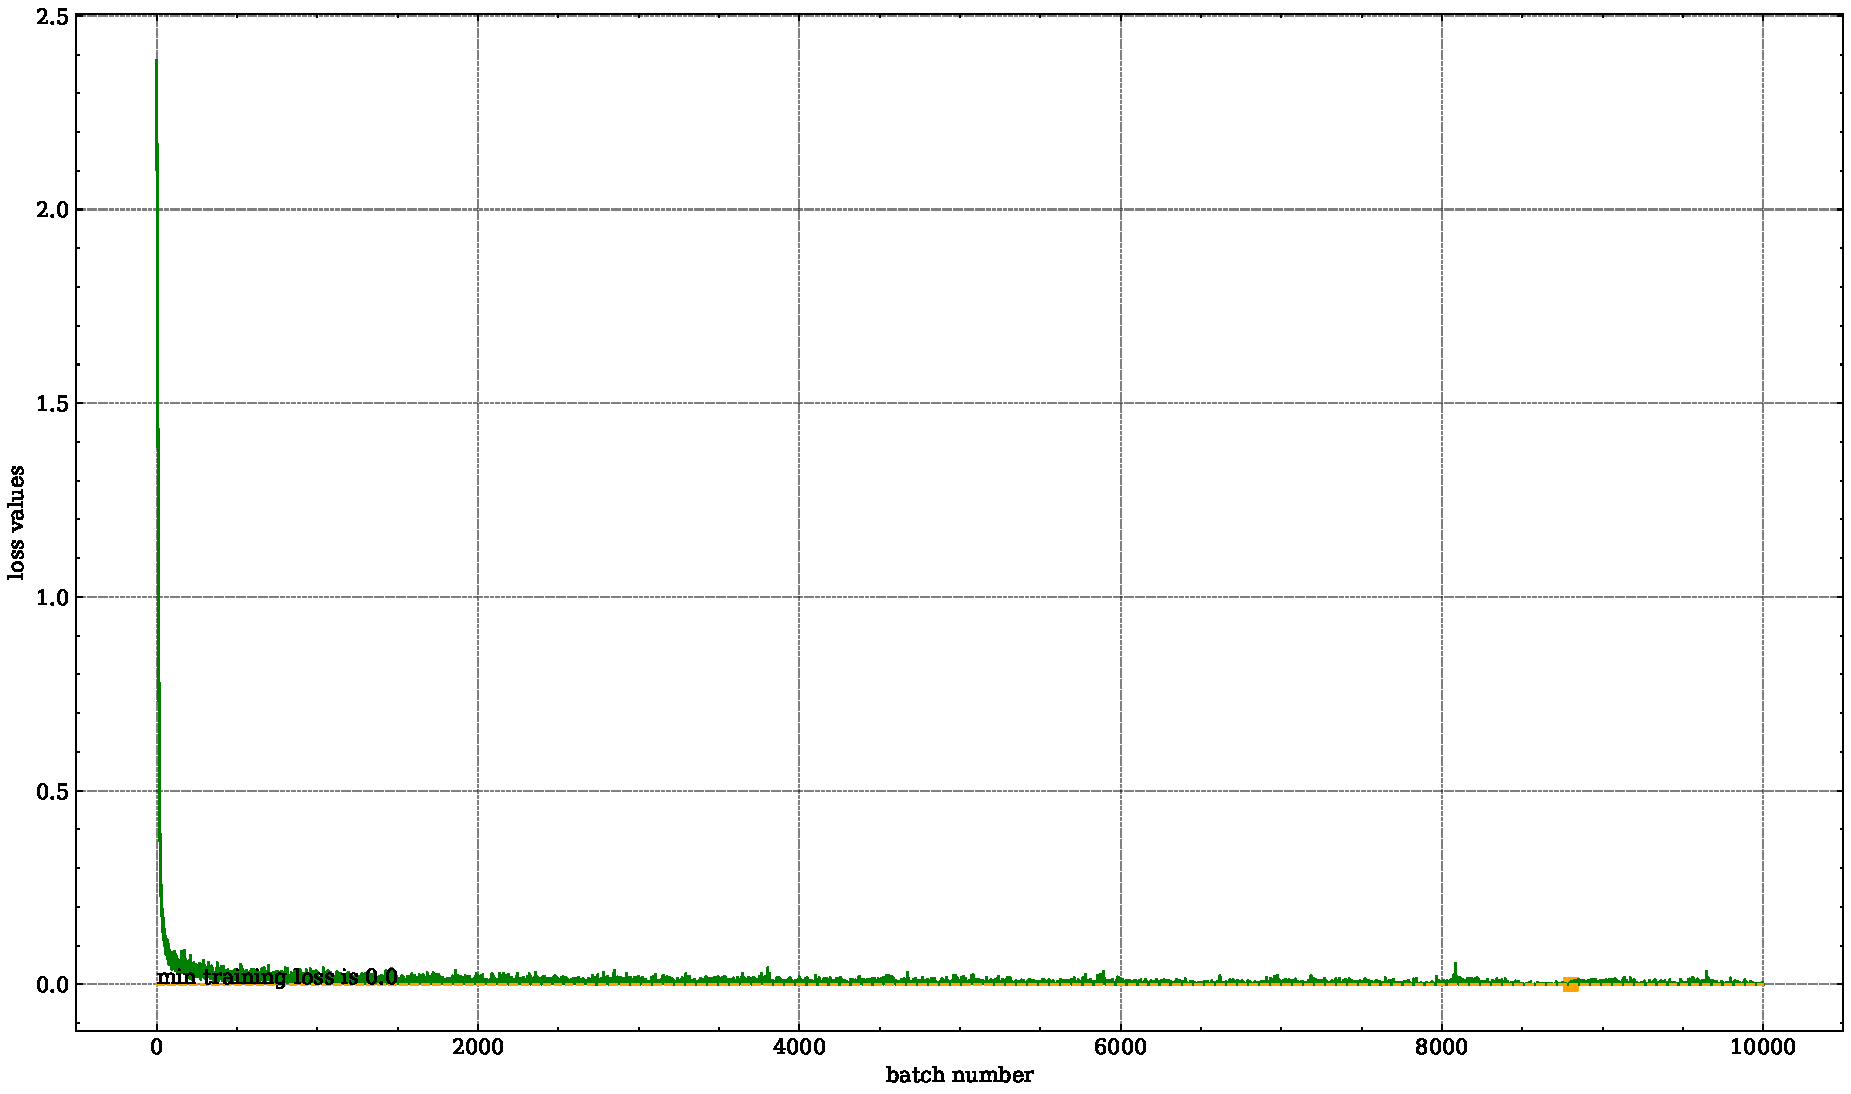
\includegraphics[scale=0.45]{../images/ResNet18训练损失函数batch.pdf}
		\caption{ResNet18训练损失函数变化图}
		\label{ResNet18训练损失函数batch}
	\end{center}
\end{figure}
\begin{figure}[H]
	\begin{center}
		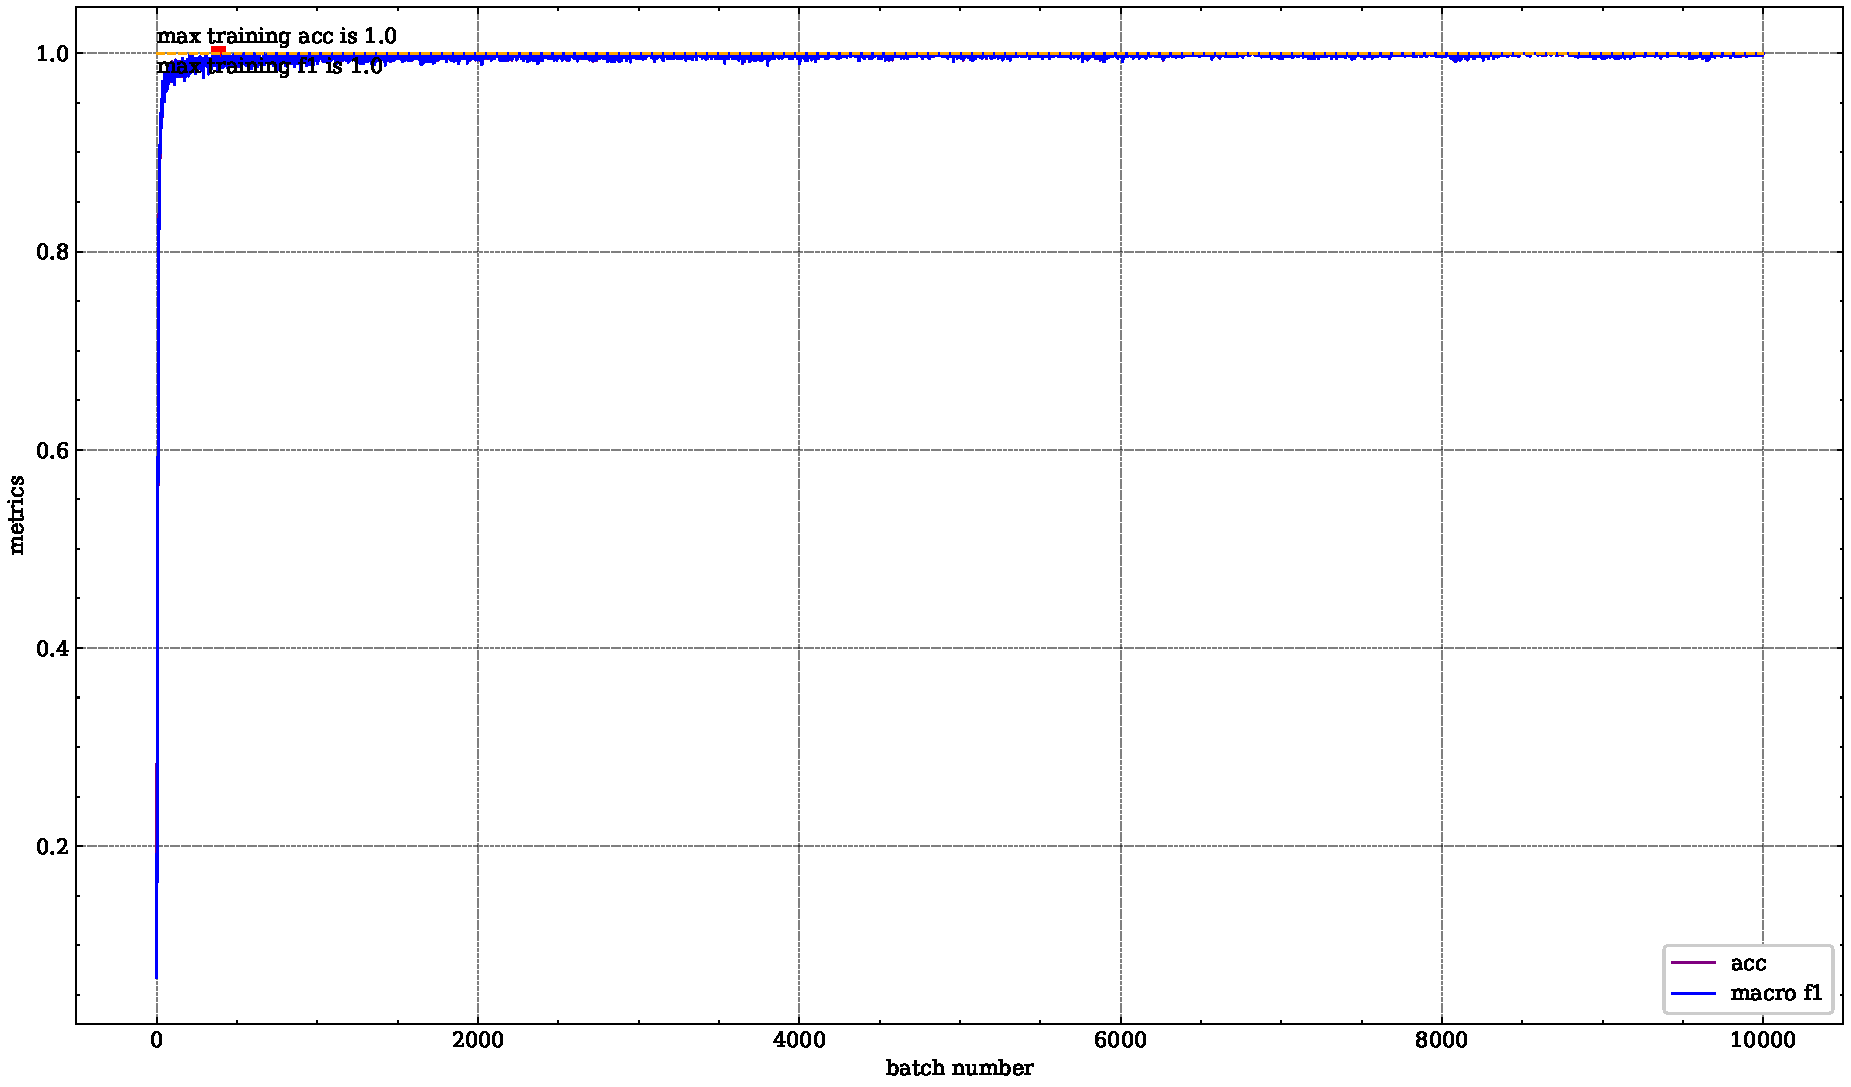
\includegraphics[scale=0.45]{../images/ResNet18训练评价指标batch.pdf}
		\caption{ResNet18训练评价指标变化图}
		\label{ResNet18训练评价指标batch}
	\end{center}
\end{figure}
\begin{figure}[H]
	\begin{center}
		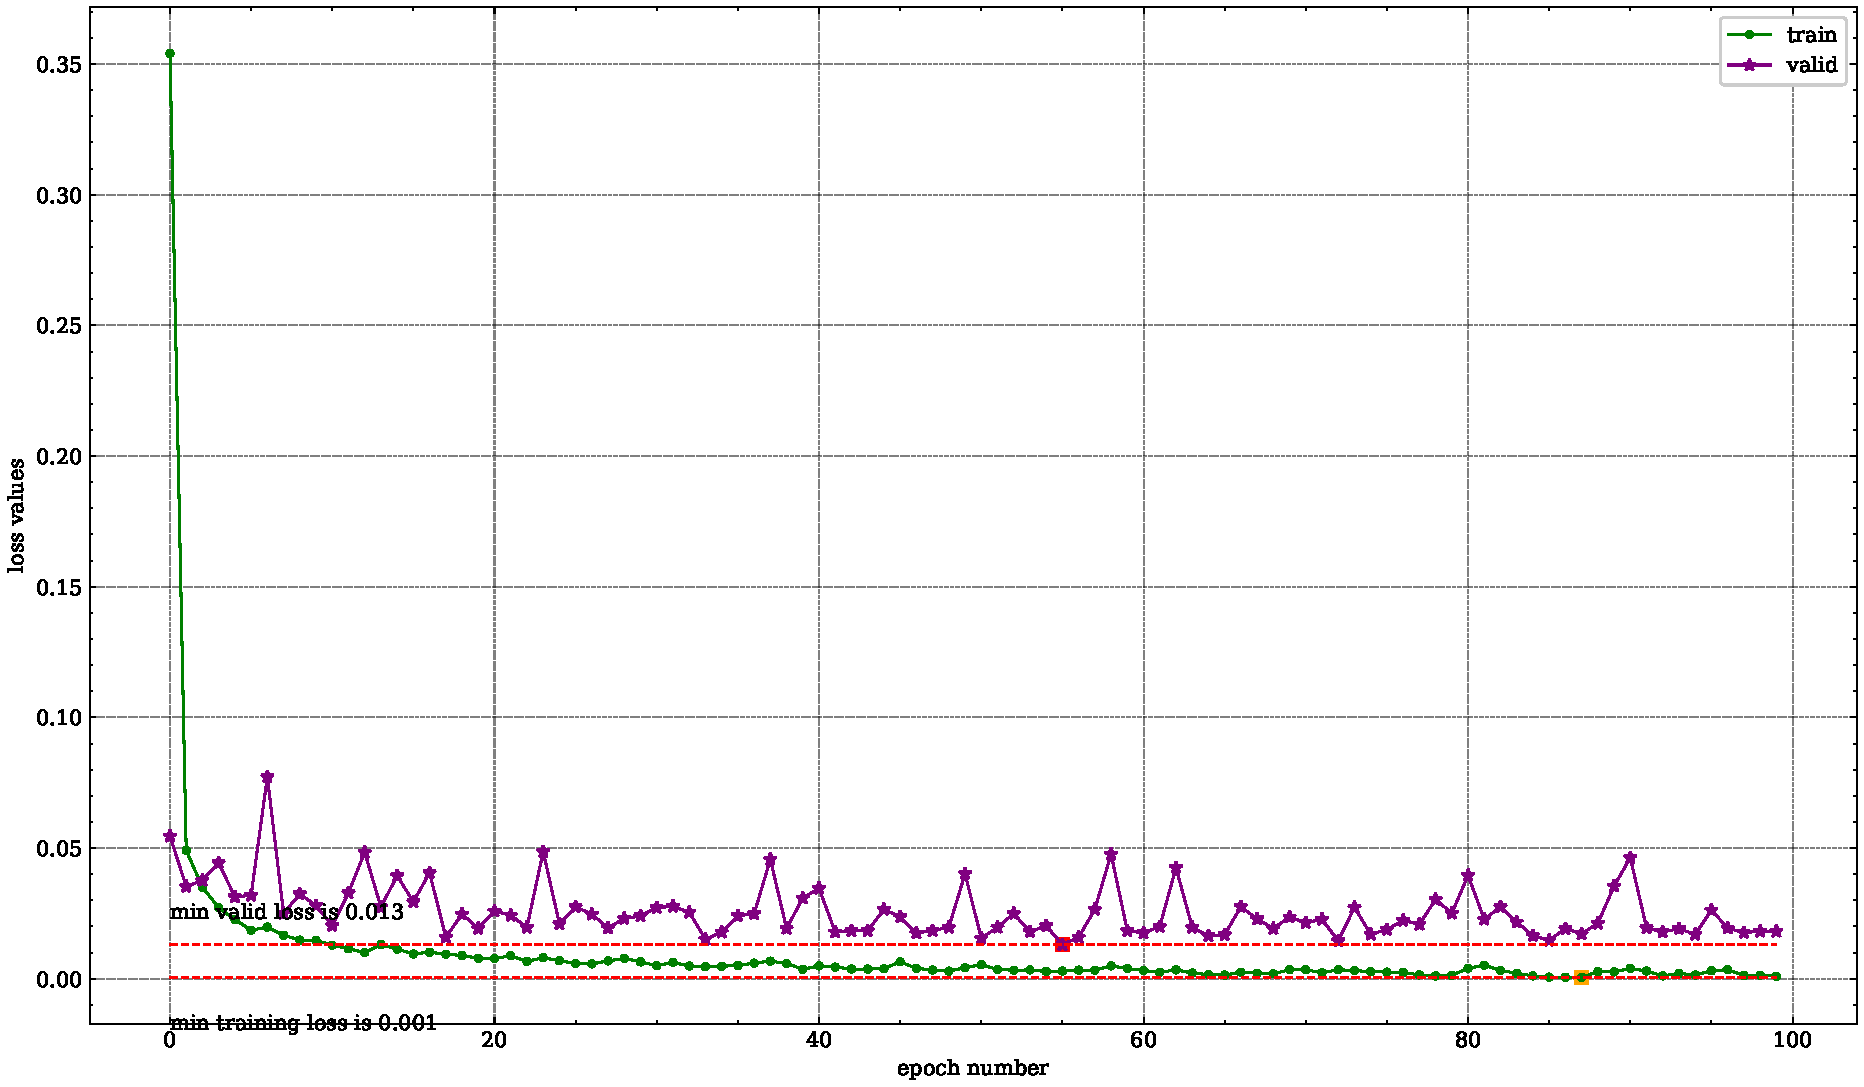
\includegraphics[scale=0.45]{../images/ResNet18训练验证损失函数.pdf}
		\caption{ResNet18 训练损失函数变化图}
		\label{ResNet18训练验证损失函数}
	\end{center}
\end{figure}
\begin{figure}[H]
	\begin{center}
		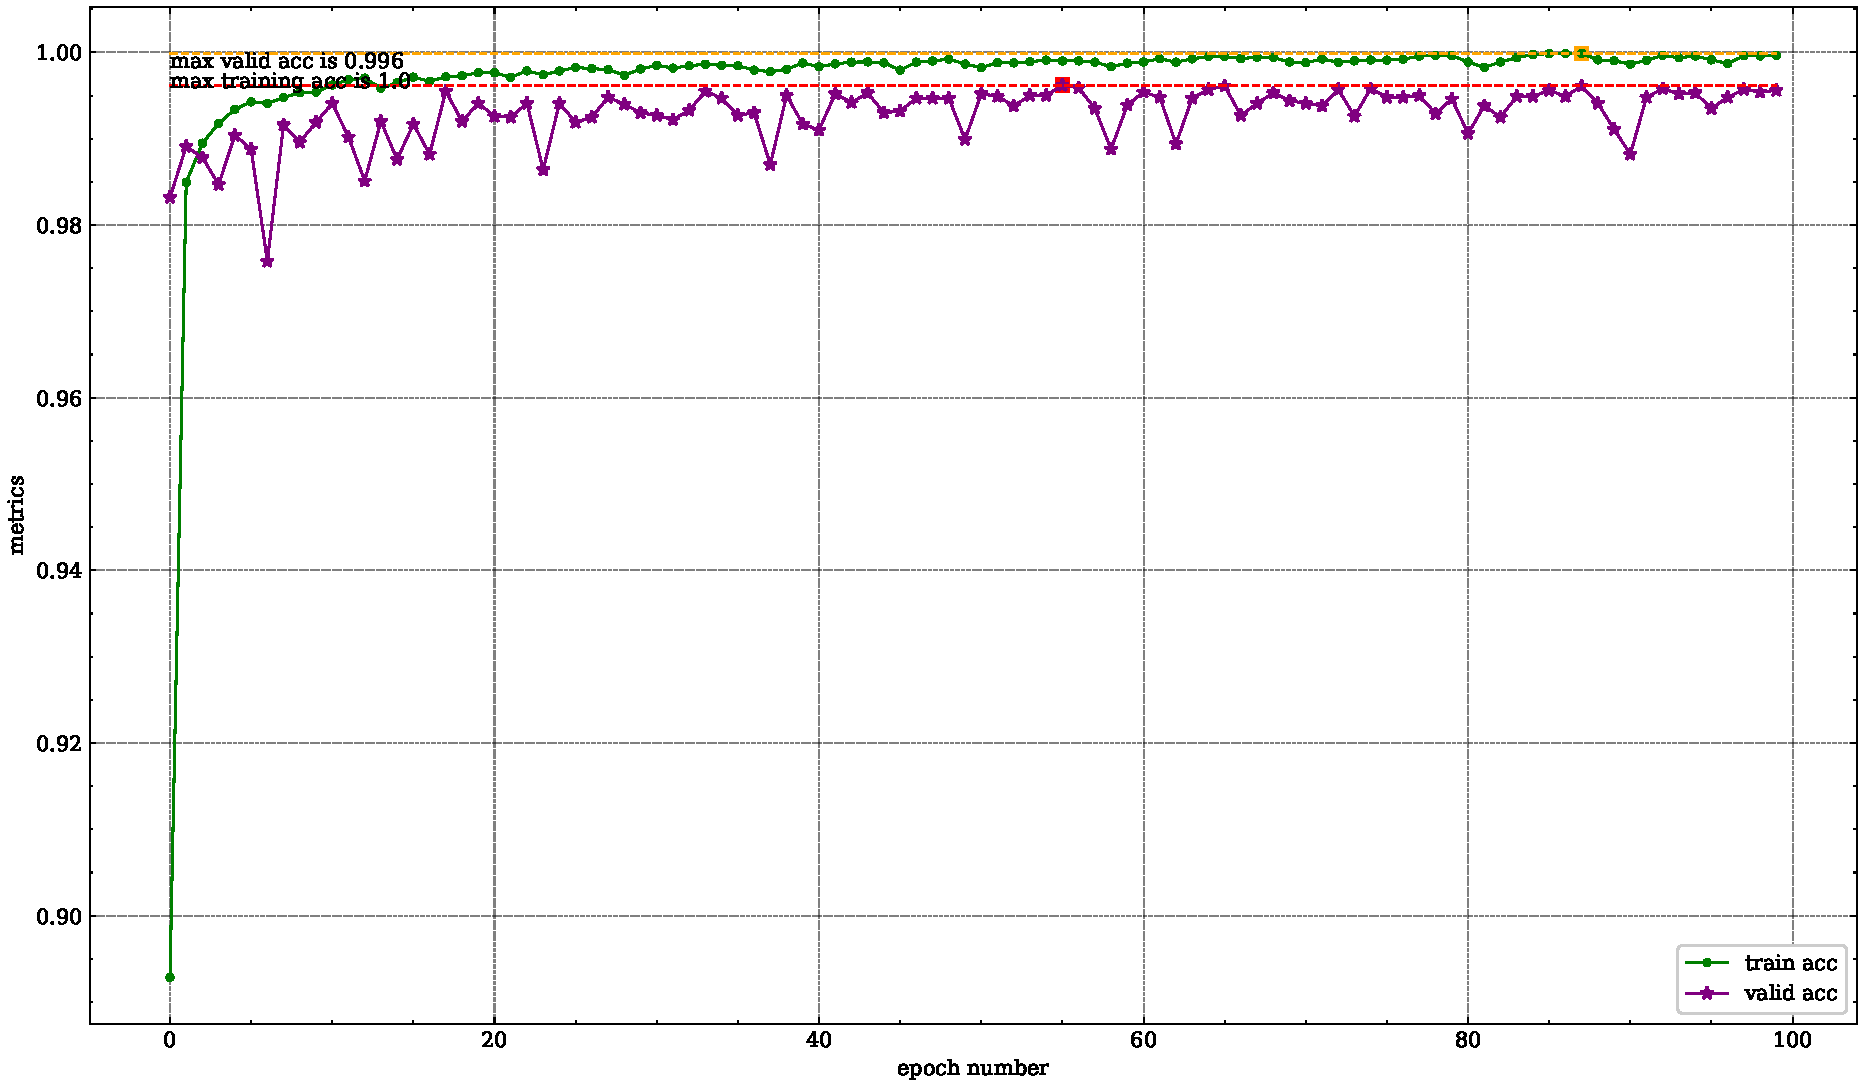
\includegraphics[scale=0.4]{../images/ResNet18训练验证acc.pdf}
		\caption{ResNet18 验证准确率变化图}
		\label{ResNet18训练验证acc}
	\end{center}
\end{figure}
\begin{figure}[H]
	\begin{center}
		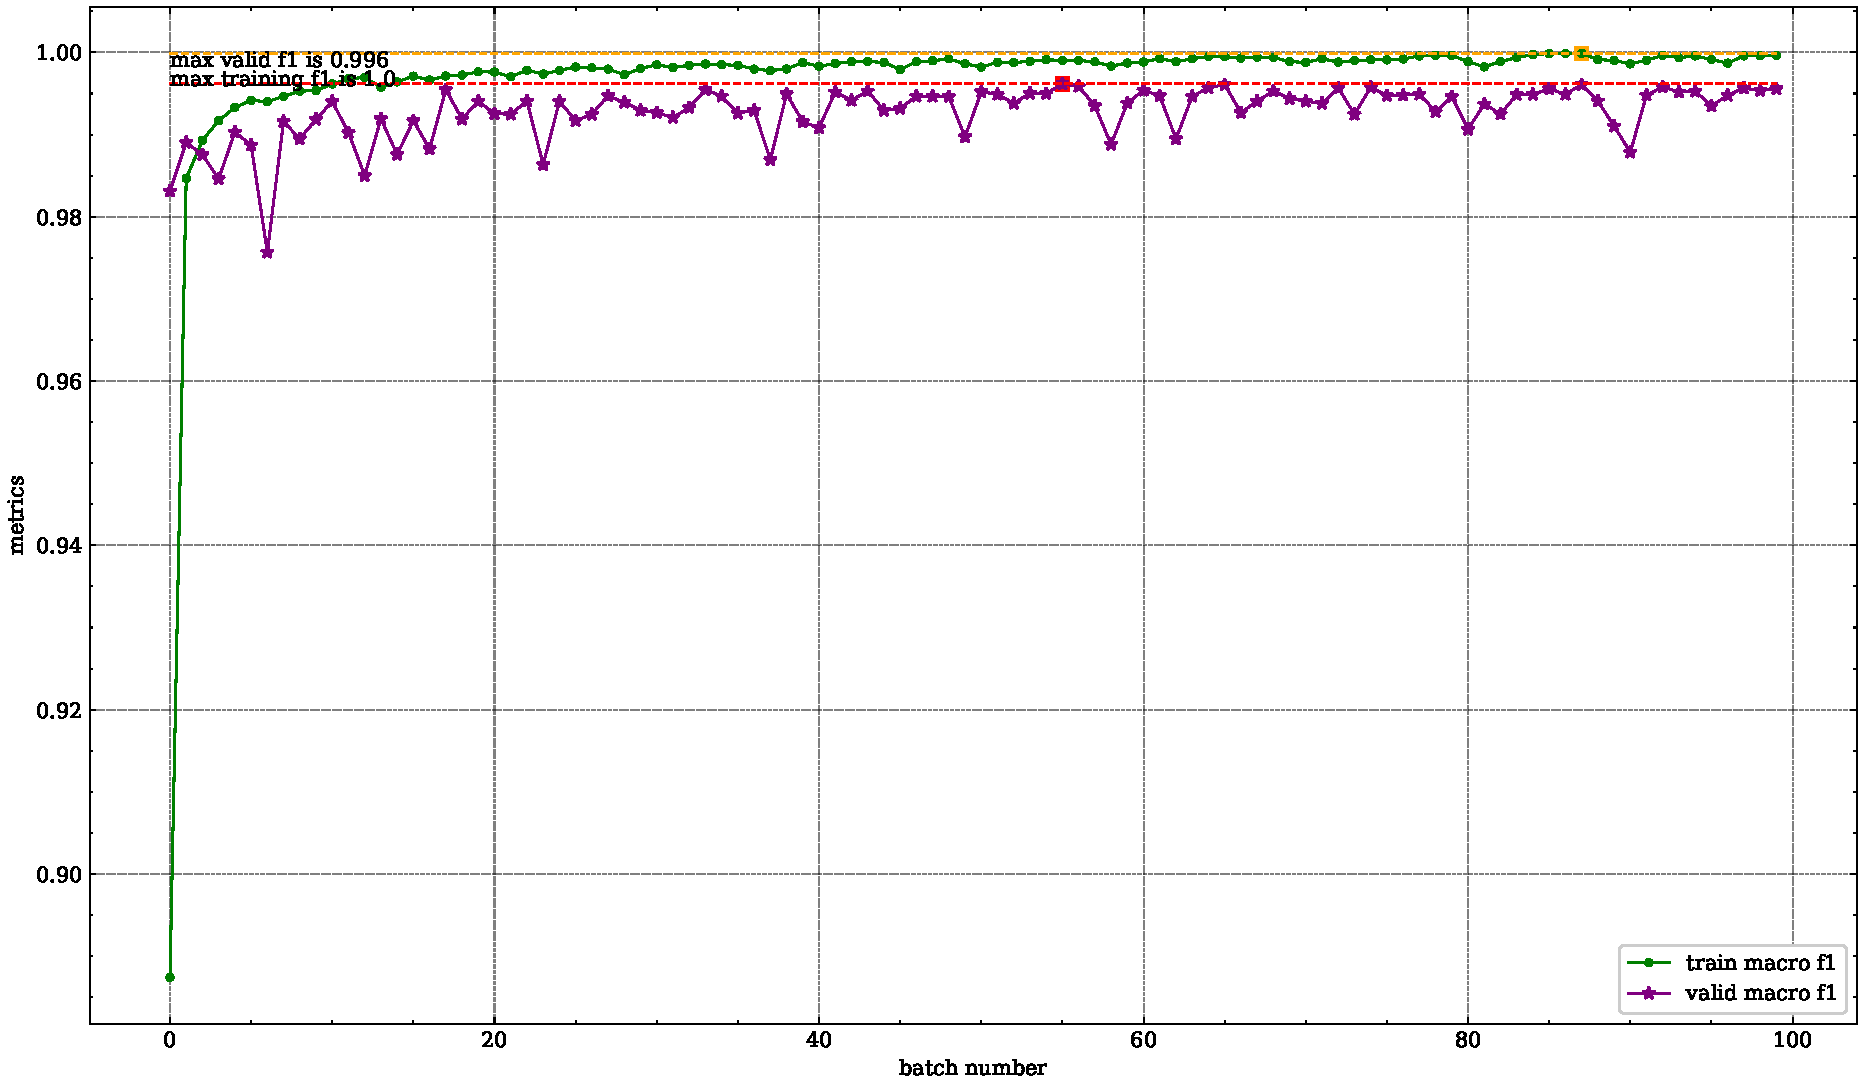
\includegraphics[scale=0.4]{../images/ResNet18训练验证f1.pdf}
		\caption{ResNet18 验证 macro f1 分数变化图}
		\label{ResNet18训练验证f1}
	\end{center}
\end{figure}

训练完成后,我们分别加载两个模型保存的最优参数进行测试。
在测试中,LeNet\_RB 模型在训练集上的准确率达到了 1.0,marco f1 分数也达到了 1.0;在验证集上的准确率达到了 0.991,marco f1 分数也达到了 0.991。
ResNet18 模型在训练集上的准确率达到了 1.0,marco f1 分数也达到了 1.0;在验证集上的准确率达到了 0.996,marco f1 分数也达到了 0.996。
两种模型的各类别的相关评价指标如表\ref{LeNetRB各类别评价指标}和\ref{ResNet18各类别评价指标}所示。
\begin{table}[H]
	\centering
	\caption{LeNet\_RB 各类别的评价指标}
	  \begin{tabular}{ccccc}
		\toprule
			& \textbf{precision} & \textbf{recall} & \textbf{f1-score} & \textbf{support} \\\hline
	  \textbf{0} & 0.99  & 0.99  & 0.99  & 980 \\
	  \textbf{1} & 0.99  & 1     & 0.99  & 1135 \\
	  \textbf{2} & 0.99  & 0.99  & 0.99  & 1032 \\
	  \textbf{3} & 0.99  & 0.99  & 0.99  & 1010 \\
	  \textbf{4} & 0.99  & 0.99  & 0.99  & 982 \\
	  \textbf{5} & 0.99  & 0.99  & 0.99  & 892 \\
	  \textbf{6} & 1     & 0.99  & 0.99  & 958 \\
	  \textbf{7} & 0.98  & 1     & 0.99  & 1028 \\
	  \textbf{8} & 1     & 0.98  & 0.99  & 974 \\
	  \textbf{9} & 0.99  & 0.98  & 0.99  & 1009 \\
	  \textbf{accuracy} &       &       & 0.99  & 10000 \\
	  \textbf{macro avg} & 0.99  & 0.99  & 0.99  & 10000 \\
	  \textbf{weighted avg} & 0.99  & 0.99  & 0.99  & 10000 \\\bottomrule
	  \end{tabular}
	\label{LeNetRB各类别评价指标}
  \end{table}
  \begin{table}[H]
	\centering
	\caption{ResNet18 各类别的评价指标}
	  \begin{tabular}{ccccc}
		\toprule
			& \textbf{precision} & \textbf{recall} & \textbf{f1-score} & \textbf{support} \\\hline
	  \textbf{0} & 1  & 1  & 1  & 980 \\
	  \textbf{1} & 1  & 1     & 1  & 1135 \\
	  \textbf{2} & 0.99  & 1  & 1  & 1032 \\
	  \textbf{3} & 0.99  & 1  & 1  & 1010 \\
	  \textbf{4} & 0.99  & 0.99  & 0.99  & 982 \\
	  \textbf{5} & 0.99  & 0.99  & 0.99  & 892 \\
	  \textbf{6} & 1     & 0.99  & 1  & 958 \\
	  \textbf{7} & 1  & 0.99     & 0.99  & 1028 \\
	  \textbf{8} & 1     & 1  & 1  & 974 \\
	  \textbf{9} & 0.99  & 0.99  & 0.99  & 1009 \\
	  \textbf{accuracy} &       &       & 1  & 10000 \\
	  \textbf{macro avg} & 1  & 1  & 1  & 10000 \\
	  \textbf{weighted avg} & 1  & 1  & 1  & 10000 \\\bottomrule
	  \end{tabular}
	\label{ResNet18各类别评价指标}
  \end{table}

\section{总结与讨论}
在这一章,我们研究了不同的网络架构和不同超参数变化对模型准确率的影响。结果如下。

\subsection{两种不同架构模型之间的对比}
我们将 LeNet\_RB 和 ResNet18 两种模型的验证评价指标、训练损失函数变化和评价指标变化进行了对比。

首先我们对比模型在验证集上的表现。两种模型在验证集上的最小损失函数值、准确率和 macro f1 分数如表\ref{模型对比表}所示。
\begin{table}[H]
	\centering
	\caption{模型效果对比表}
	  \begin{tabular}{cccc}
		\toprule
			& \textbf{最小验证损失函数值} & \textbf{准确率} & \textbf{macro f1 分数} \\\hline
	  \textbf{LeNet\_RB} & 0.029 & 0.991 & 0.991 \\
	  \textbf{ResNet18} & 0.013 & 0.996 & 0.996 \\
	  \bottomrule
	  \end{tabular}
	\label{模型对比表}
  \end{table}

接着,我们对比两者在训练集上的最小损失函数值和准确率,如图\ref{损失函数对比}和图\ref{准确率对比}所示。
\begin{figure}[H]
	\begin{center}
		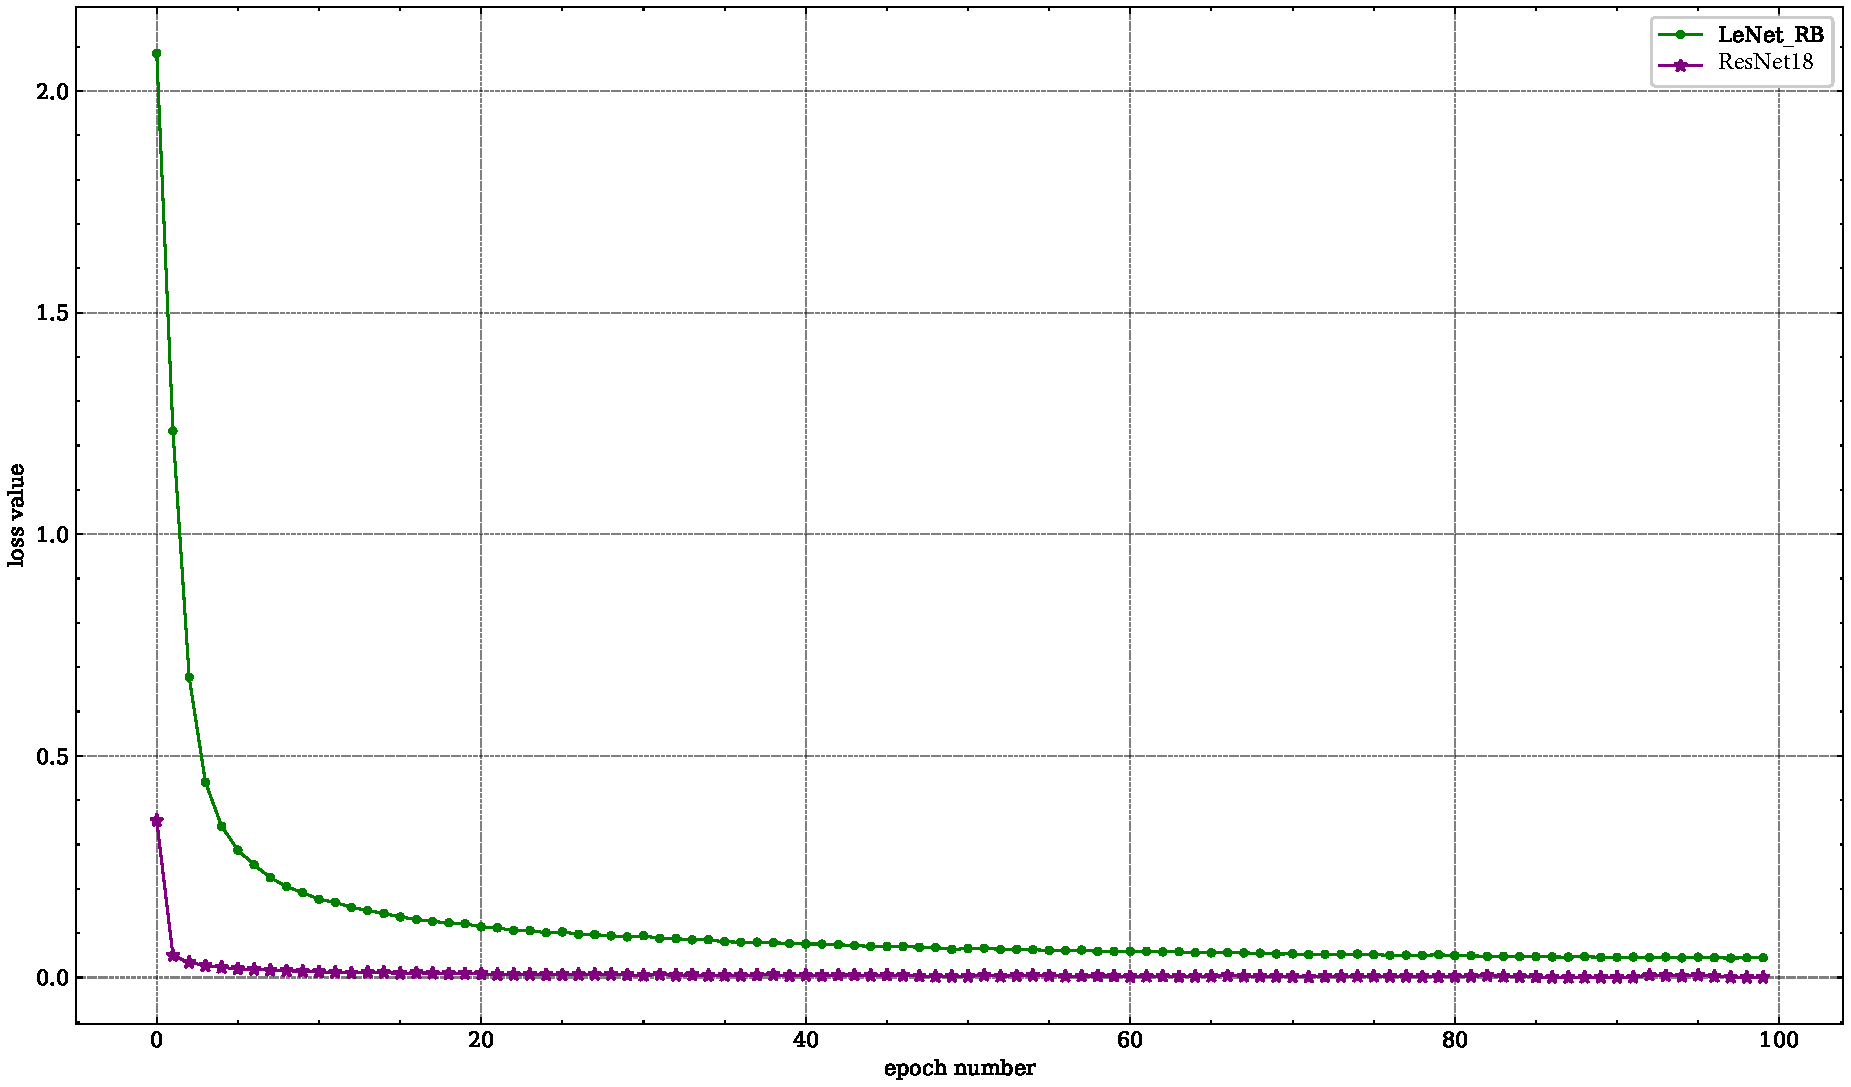
\includegraphics[scale=0.45]{../images/模型对比loss.pdf}
		\caption{两种模型的训练集损失函数值对比}
		\label{损失函数对比}
	\end{center}
\end{figure}
\begin{figure}[H]
	\begin{center}
		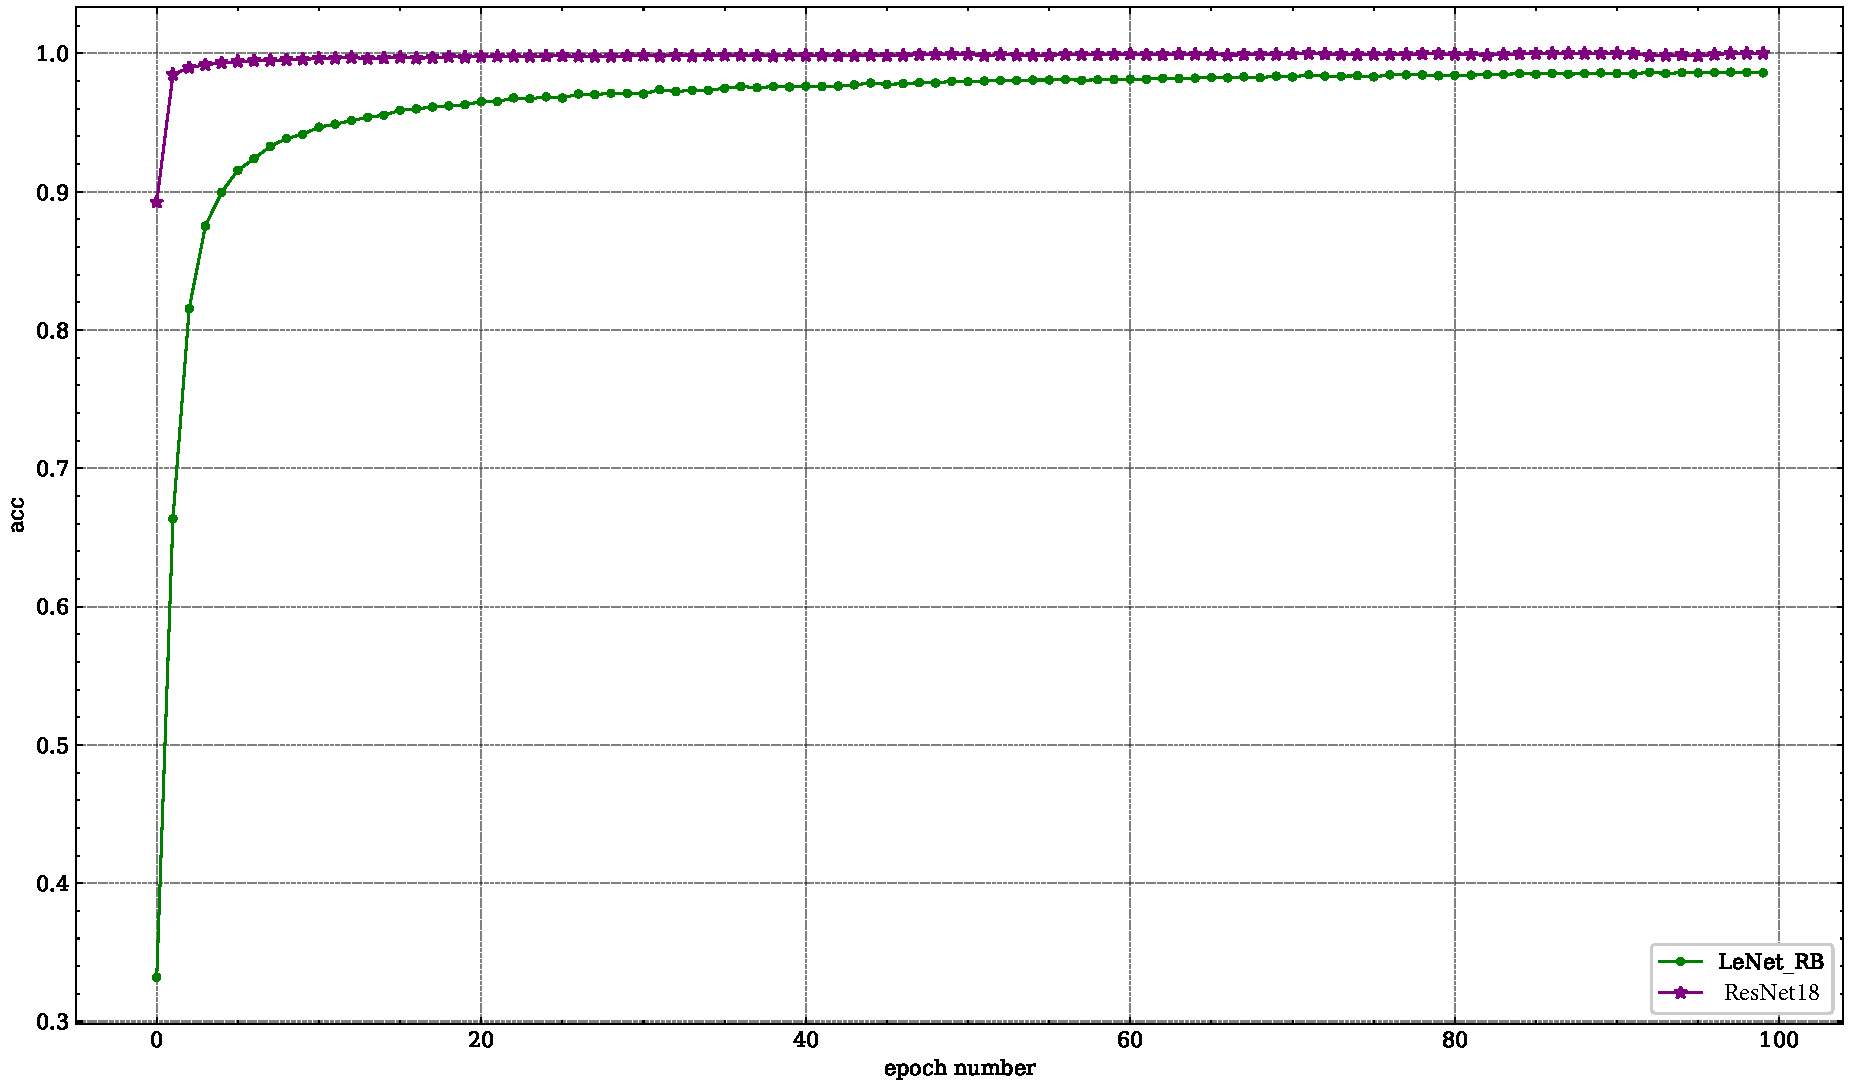
\includegraphics[scale=0.45]{../images/模型对比acc.pdf}
		\caption{两种模型的训练集准确率对比}
		\label{准确率对比}
	\end{center}
\end{figure}
  
我们发现,无论是在训练集还是验证集上,ResNet18 的相关指标均略优于 LeNet\_RB。这是由于 ResNet18 的网络层数较多,表达能力较强。
但是,两种模型在验证集上的准确率差别并没有特别大,而 LeNet\_RB 由于参数较少,其训练和推理用时均明显少于 ResNet18。所以,综合准确率和时间因素
LeNet\_RB 是一个更好的选择。
\subsection{不同的学习率对准确率的影响}
我们保持除学习率和最大训练轮数外的其它超参数不变,
依次将学习率设置成 $10^{-6}, 10^{-5}, ..., 1, 10$。
并适当调整最大训练轮数使得使得每个网络的效果均达到最优。
接着对每个网络进行训练并测试其准确率。
对于 LeNet\_RB,其结果如图\ref{LeNetRB不同的学习率}所示。
\begin{figure}[H]
	\begin{center}
		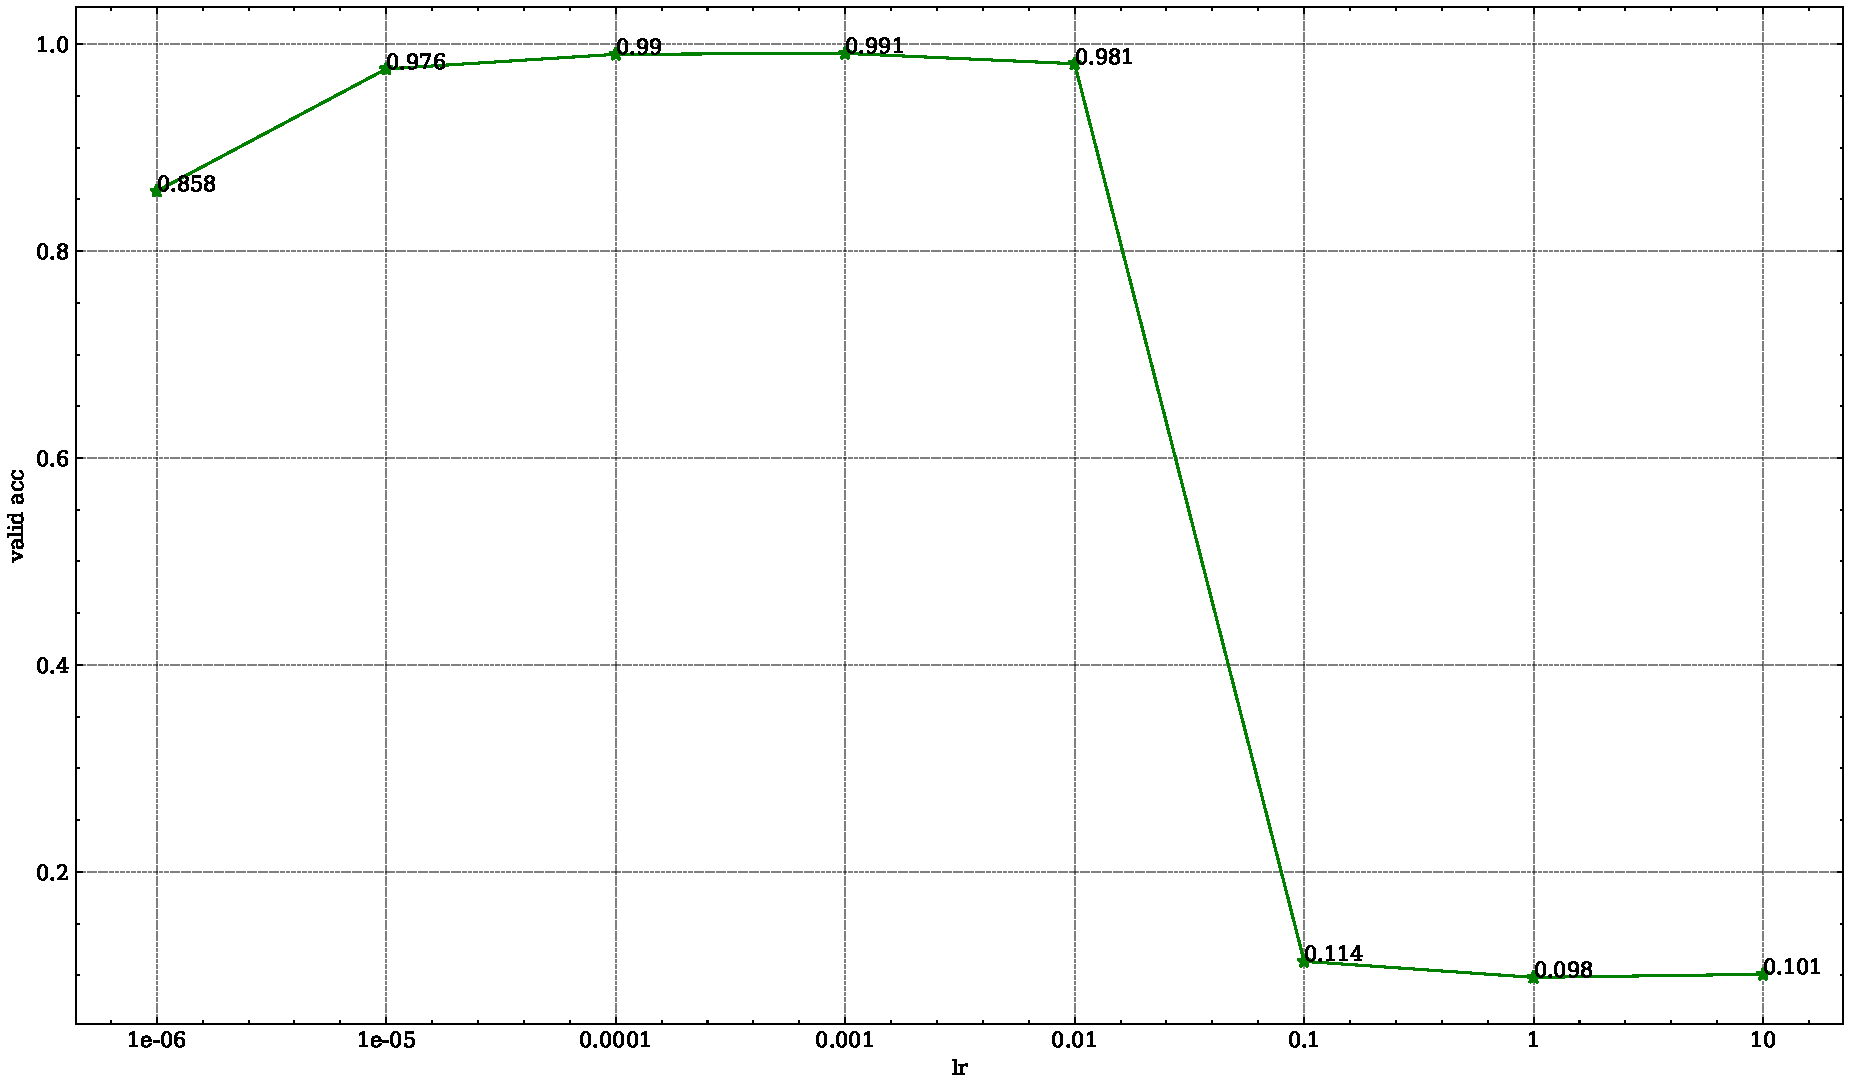
\includegraphics[scale=0.4]{../images/LeNetRB不同的学习率.pdf}
		\caption{LeNet\_RB 模型不同的学习率对准确率的影响}
		\label{LeNetRB不同的学习率}
	\end{center}
\end{figure}

对于 ResNet18,其结果如图\ref{ResNet18不同的学习率}所示。
\begin{figure}[H]
	\begin{center}
		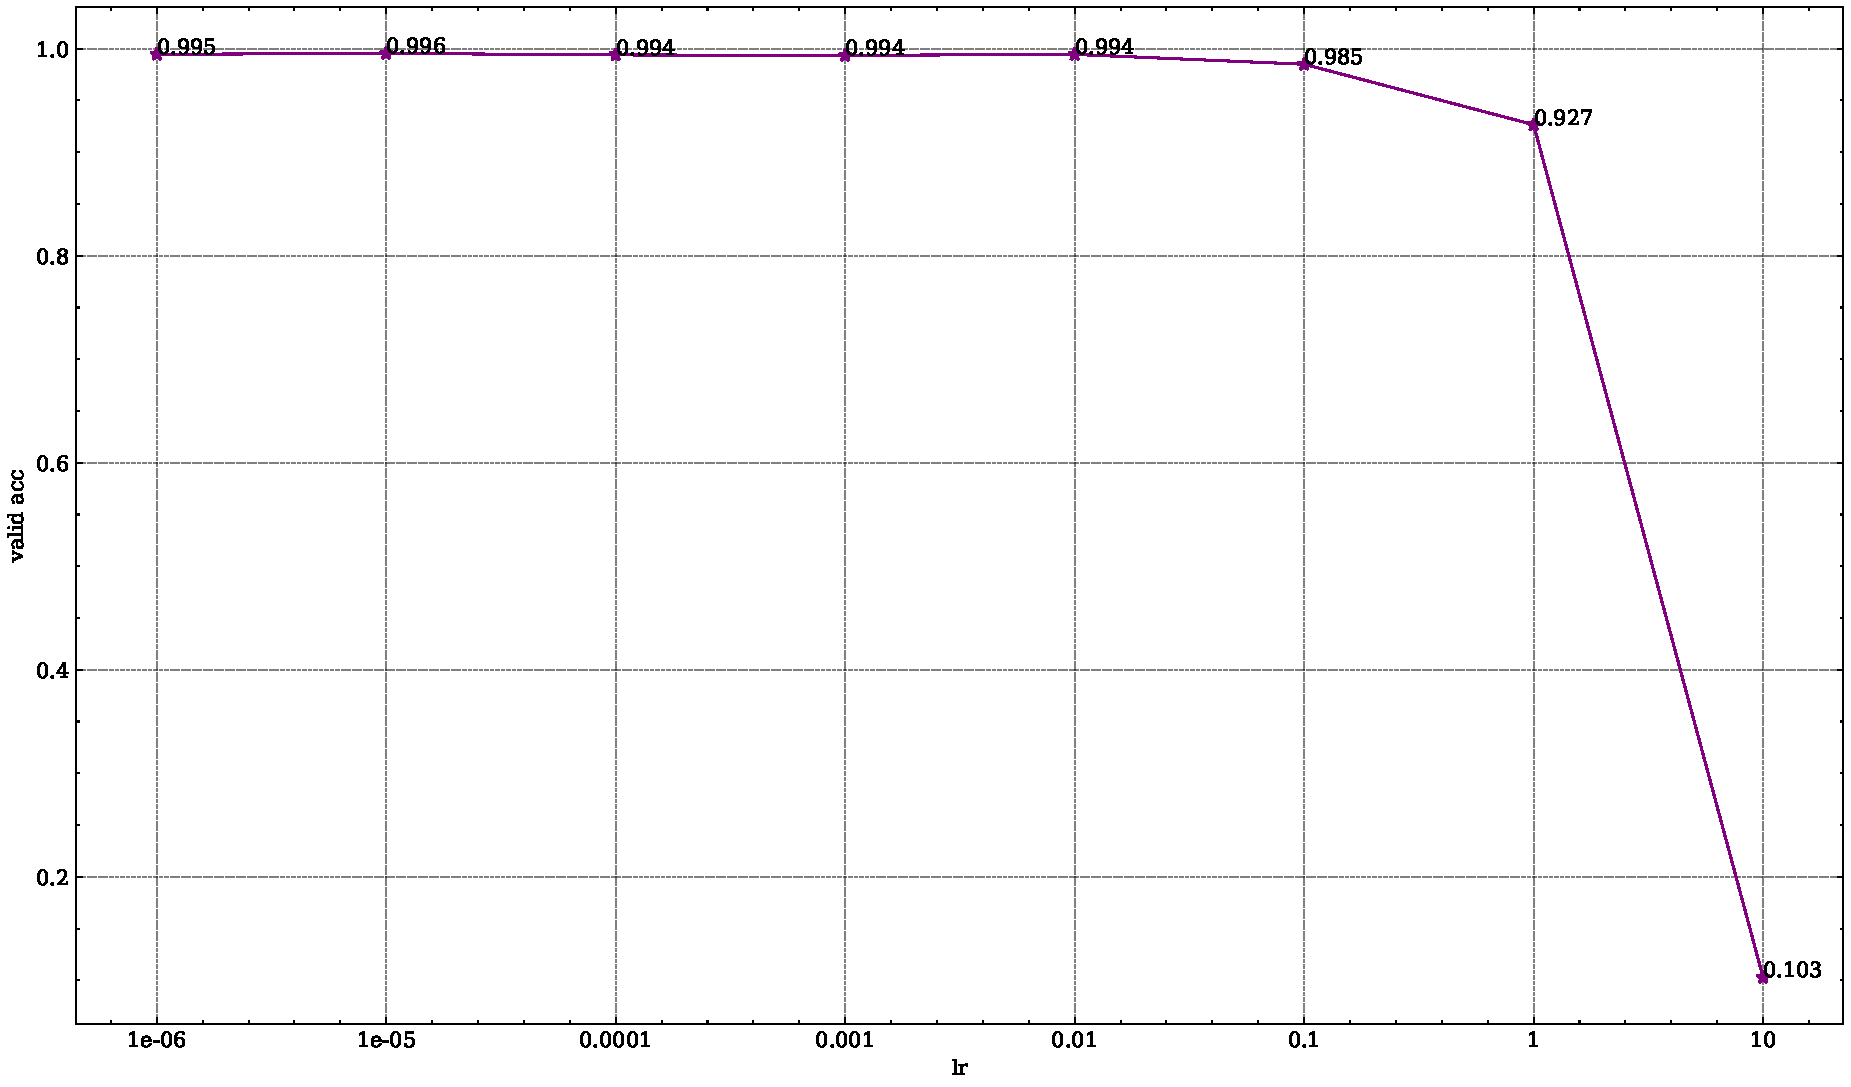
\includegraphics[scale=0.4]{../images/ResNet18不同的学习率.pdf}
		\caption{ResNet18 模型不同的学习率对准确率的影响}
		\label{ResNet18不同的学习率}
	\end{center}
\end{figure}

从图\ref{LeNetRB不同的学习率}和图\ref{ResNet18不同的学习率}中我们可以看出,随着学习率的增加,
LeNet\_RB 模型的准确率先略微上升后大幅下降,并在学习率为 0.001 时达到最优值;ResNet18 模型的准确率先保持稳定后大幅下降,并在学习率为 $10^{-5}$ 时达到最优值。
这是因为当学习率较小时,模型可能会陷入局部极小值。
所以随着学习率的增大,模型效果可能会有所提升。当学习率较大时,模型会在极小值附近震荡无法收敛。
所以随着学习率的继续增大,模型效果会明显下降。

\subsection{不同的批大小对准确率的影响}
我们保持除批大小外的其它超参数不变,
依次将批大小设置成 600, 1200, 2400, 4800, 6000(LeNet\_RB) 和 600, 1200, 2400, 3600(ResNet18)。
接着对每个网络进行训练并测试其准确率。
对于 LeNet\_RB,其结果如图\ref{LeNetRB不同的batchsize}所示。
\begin{figure}[H]
	\begin{center}
		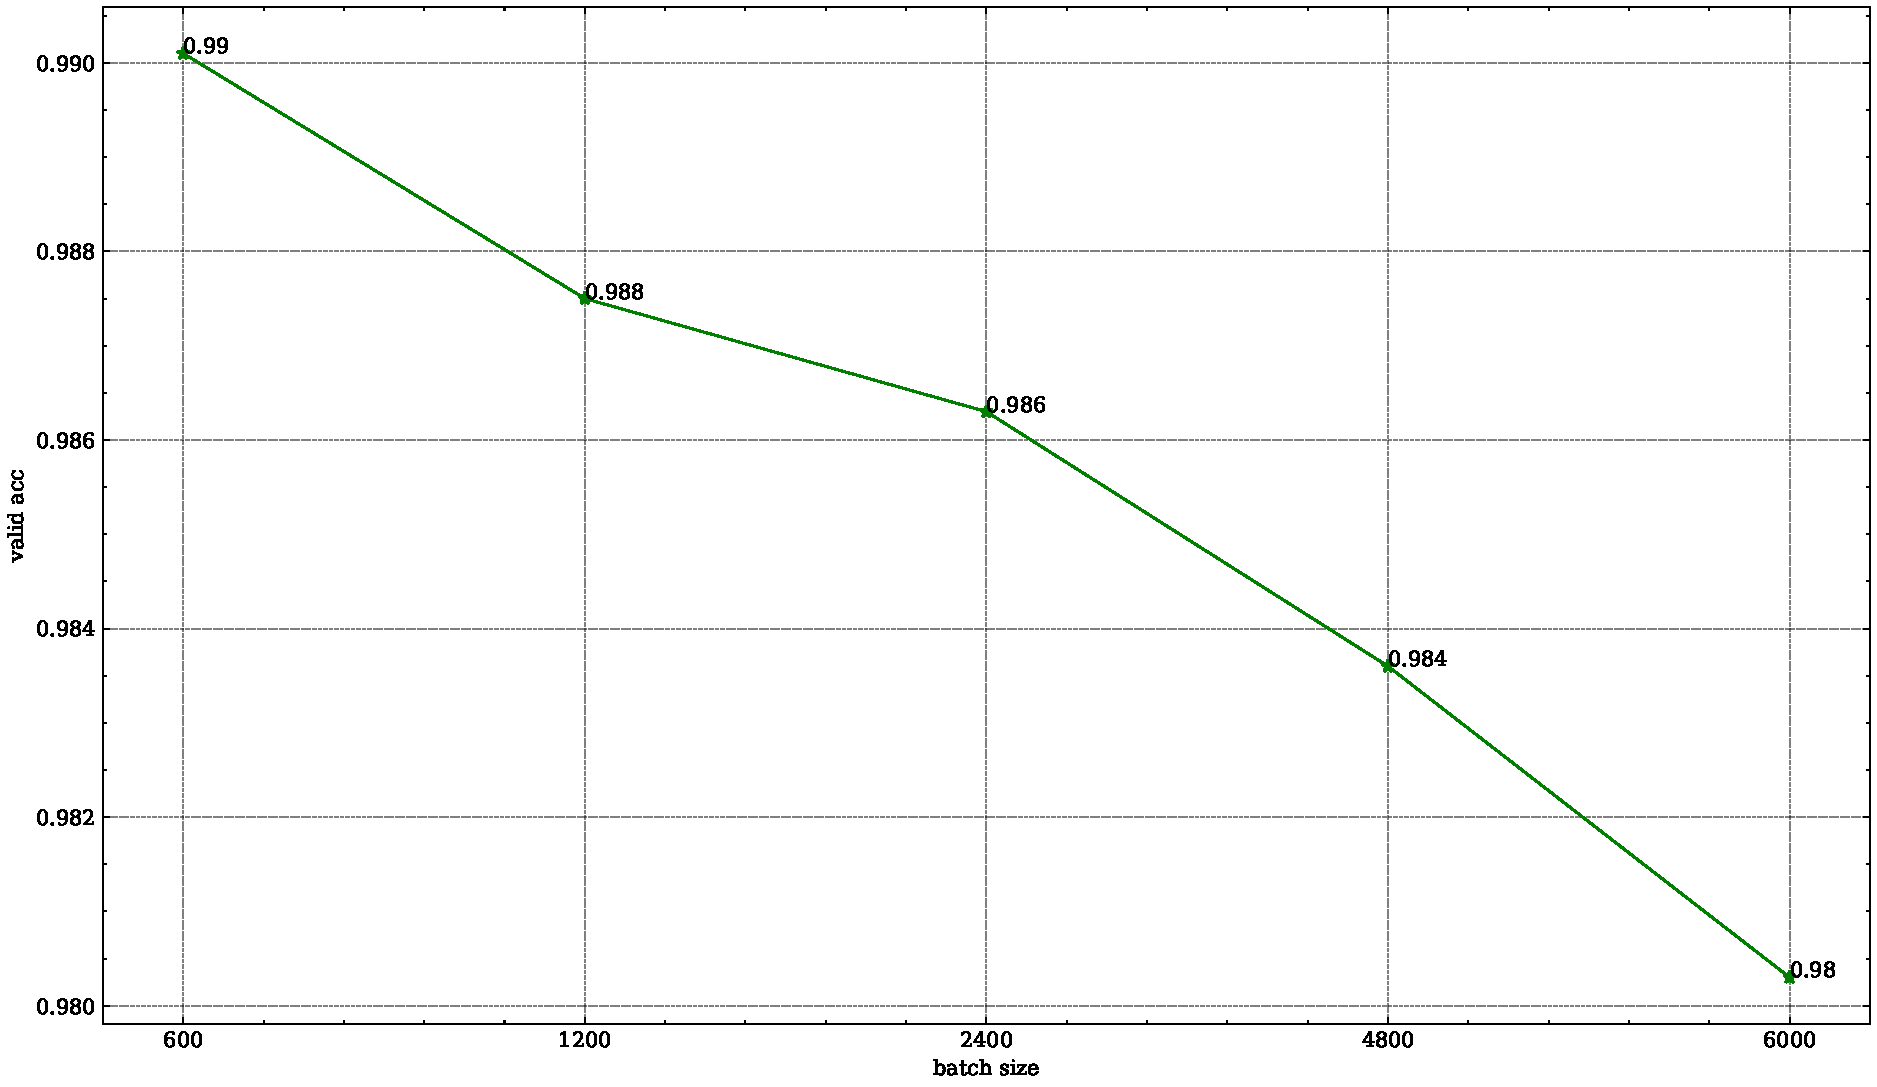
\includegraphics[scale=0.35]{../images/LeNetRB不同的batchsize.pdf}
		\caption{LeNet\_RB 模型不同的批大小对准确率的影响}
		\label{LeNetRB不同的batchsize}
	\end{center}
\end{figure}

对于 ResNet18,其结果如图\ref{ResNet18不同的batchsize}所示。
\begin{figure}[H]
	\begin{center}
		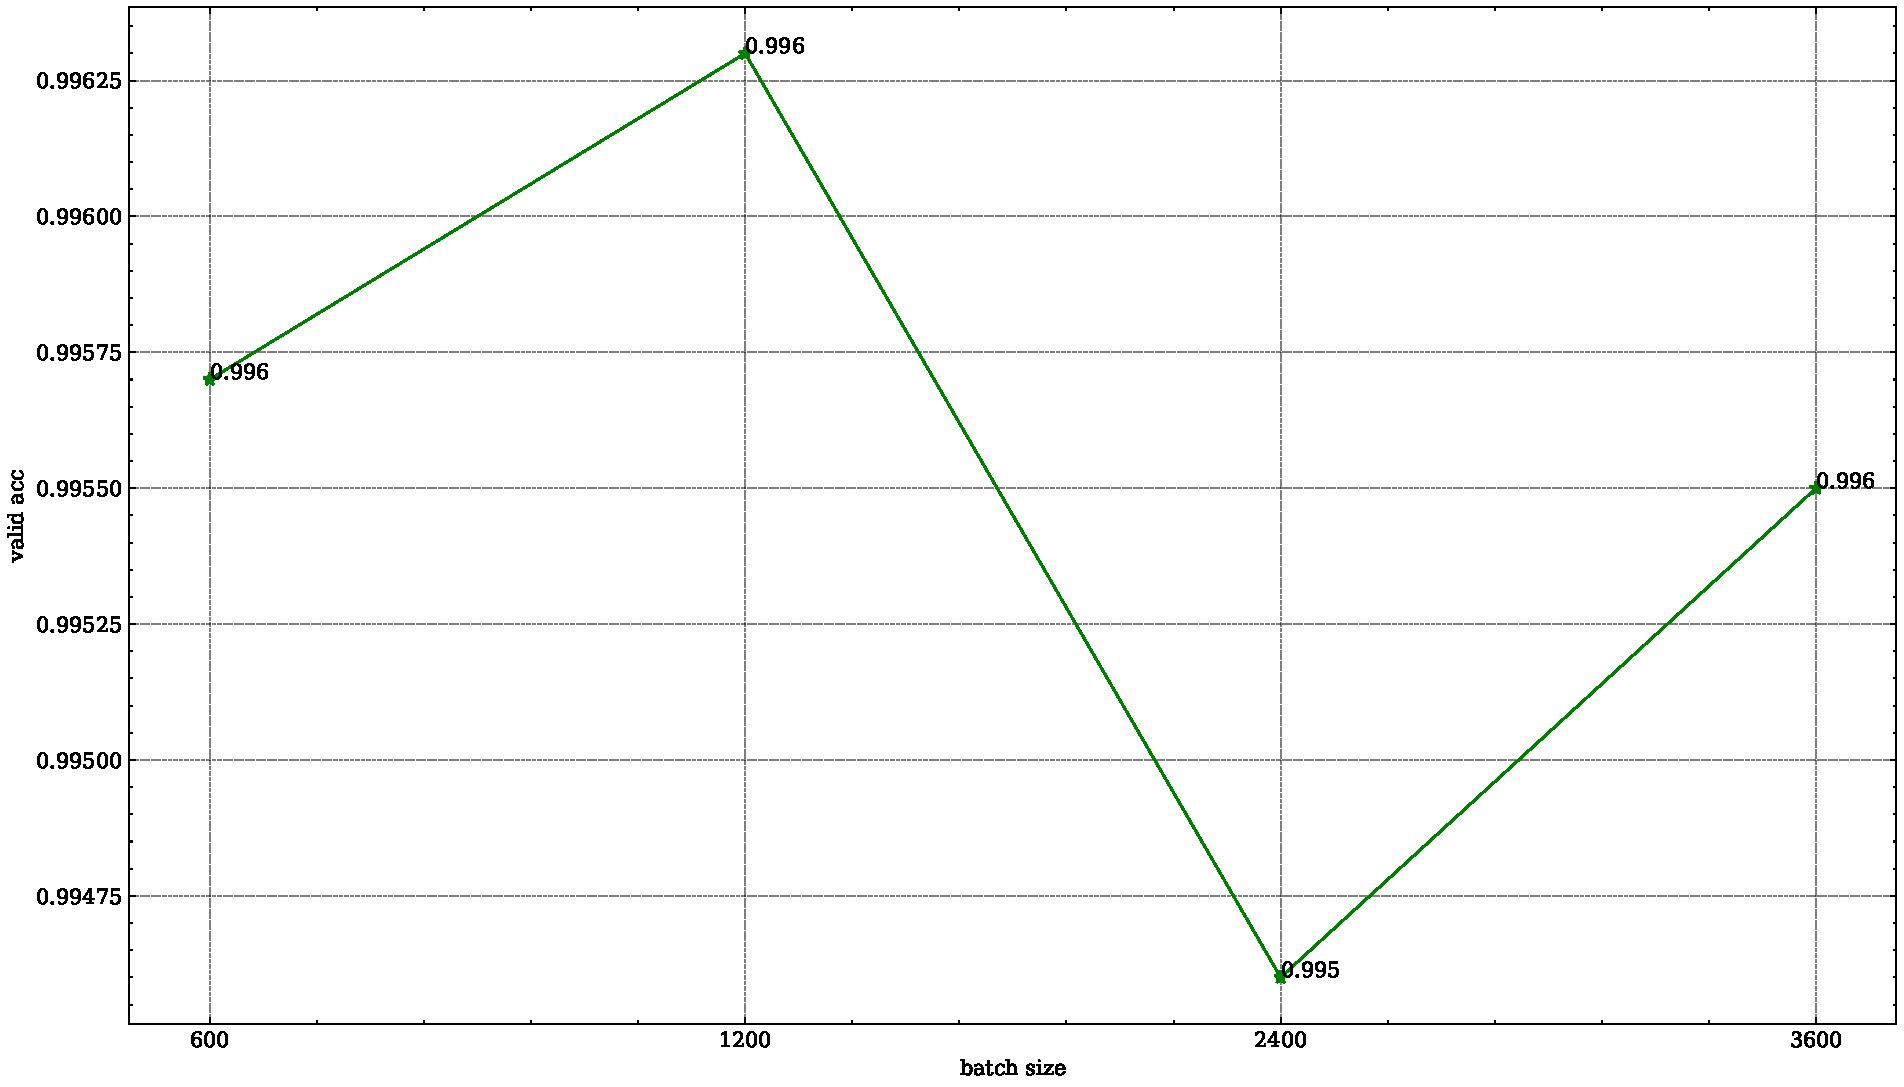
\includegraphics[scale=0.35]{../images/ResNet18不同的batchsize.pdf}
		\caption{ResNet18 模型不同的批大小对准确率的影响}
		\label{ResNet18不同的batchsize}
	\end{center}
\end{figure}

从图\ref{LeNetRB不同的batchsize}和图\ref{ResNet18不同的batchsize}中我们可以看出,随着批大小的增加,LeNet\_RB 模型的表现大致相同,但是有轻微的下降。
而 ResNet18 模型的效果几乎没有变化。
LeNet\_RB 模型的表现可能是因为较大的批大小使得模型过度学习训练集上的知识,产生了轻微的过拟合现象。

\section{实验代码简述}
在本章中,我们简要介绍实验代码的构成。更具体的介绍请见 ReadMe.md 文件。

工作目录中存在 7 个文件和 3 个目录。整个工作目录的结构如下。
\begin{figure}[H]
	\begin{center}
		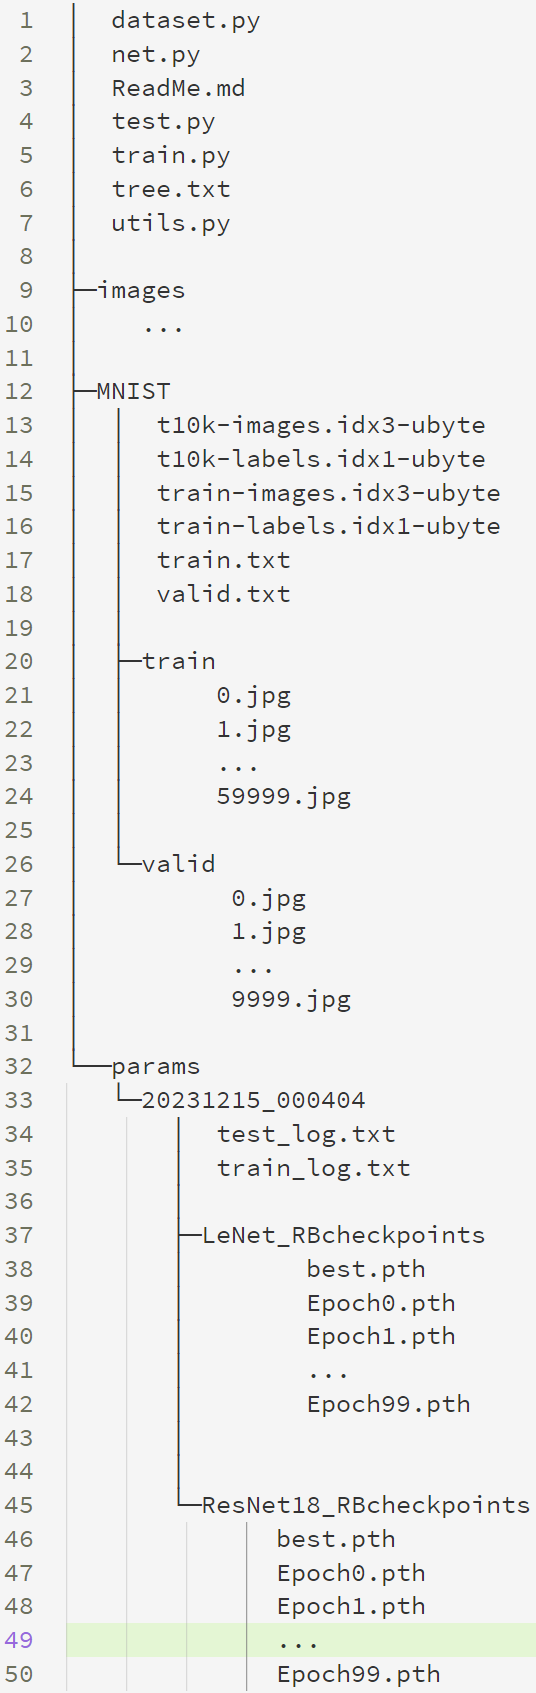
\includegraphics[scale=0.5]{../images/tree.png}
		\caption{工作目录的结构}
	\end{center}
\end{figure}

其中,dataset.csv 是原始数据集。dataset.py 中含有数据预处理的相关函数。net.py 含有模型架构的定义。
ReadMe.md 中介绍了如何对模型进行训练和测试。test.py 是进行模型测试的源代码文件。train.py是进行模型训练的源代码文件。
utils.py 中含有一些工具函数。各函数和类的源代码均含有详细的注释,方便使用者了解其完成的工作。

MNIST 目录存放数据集相关信息。images 目录存放所有绘制的图像。params 目录存放模型的参数。当在源代码中设置存储参数选项为 True 并运行一次 train.py 时,
params 目录中会增加一个以当前时间为名称的子目录。子目录内存放着训练时的日志、每一轮训练结束后的模型参数以及效果最佳的模型参数。当进行模型测试时,测试日志会放置到对应参数所在的子目录中。

\end{document}